\documentclass[../../../main]{subfiles}
\begin{document}

\section{考察}\label{sec:consideration}

\subsection{乱数生成}

\subsubsection{線形合同法の問題点}
線形合同法の問題点は、周期が短いことである。
周期の長いパラメータが提案されており、そのうちいくつかの値で乱数を生成しそのヒストグラムを作成し、
乱数の分布をみる。
乱数の生成数を$N$として$a=75, c=74, m=2^{16}+1$としたとき、そのヒストグラムを図\ref{fig:lcg-zx}に示す。
$N=2^{16}$のときは一様に分布していることがわかる。
一方で、適当な値として$s=101, c=49, m=20040213$とすると、図\ref{fig:lcg-rand}のようになる。
$N=2^{16}$のときも一様でなく出やすい値、出にくい値がでてしまうことがわかる。

線形合同法で周期の長いパラメータを発見しようとすると、
$a$、$c$、$m$の3つのパラメータを考える必要がある。
$m$が大きければ周期は大きくなる傾向にある一方で、$a$、$m$を適切に決定するためには計算量が必要となる。
全探索しようとすれば、$\mathcal{O}(n^3)$の計算量が必要となる。
これは現実的ではなく、問題点として挙げられる。

\begin{figure}
	\centering
	\begin{subfigure}{0.48\linewidth}
		\centering
		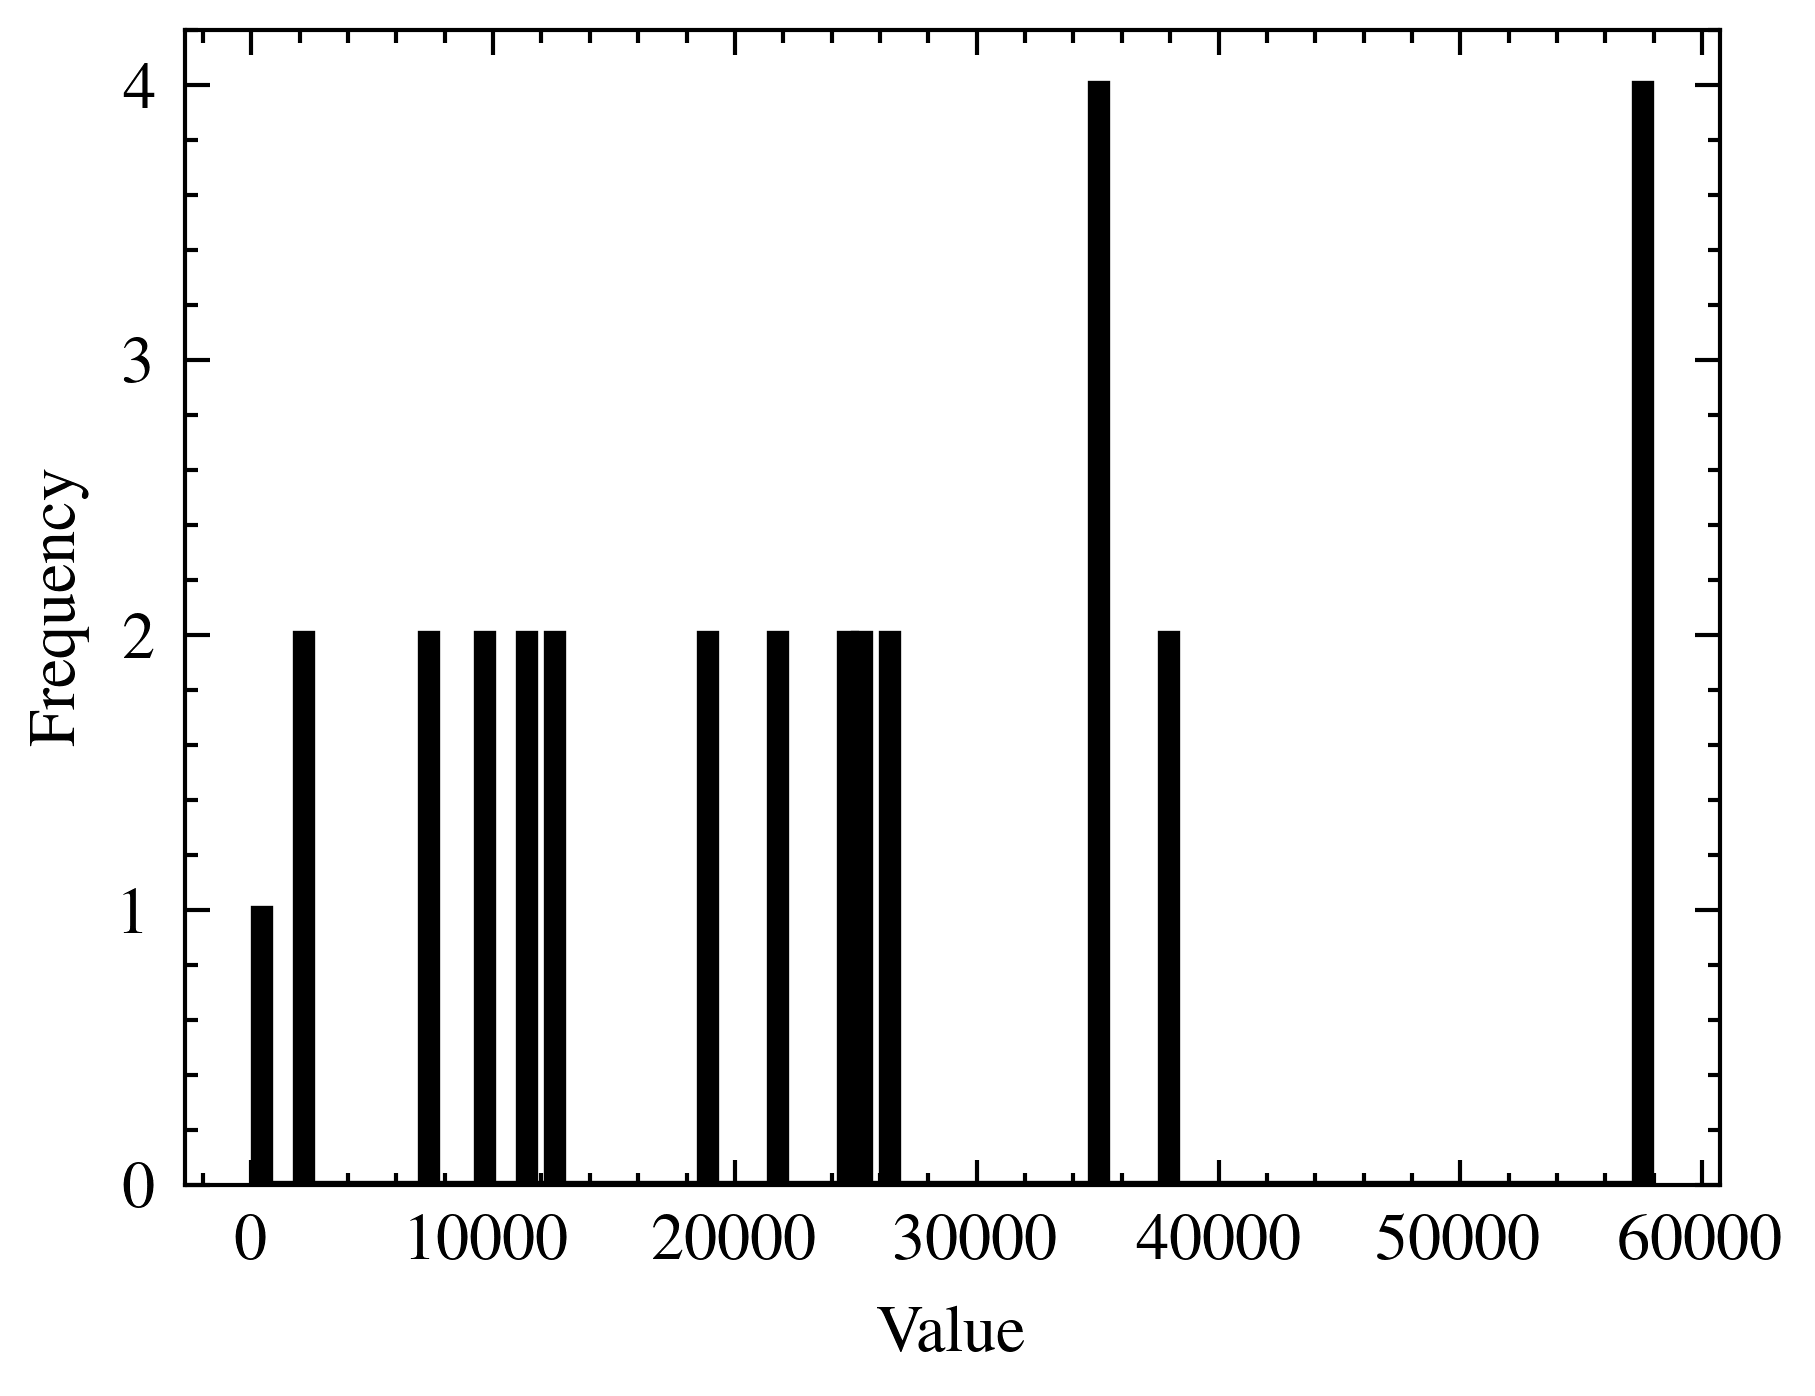
\includegraphics[width=\linewidth]{src/figures/lcg-plot/zx/lcg-2-4.png}
		\subcaption{$N=2^4$}
	\end{subfigure}
	\begin{subfigure}{0.48\linewidth}
		\centering
		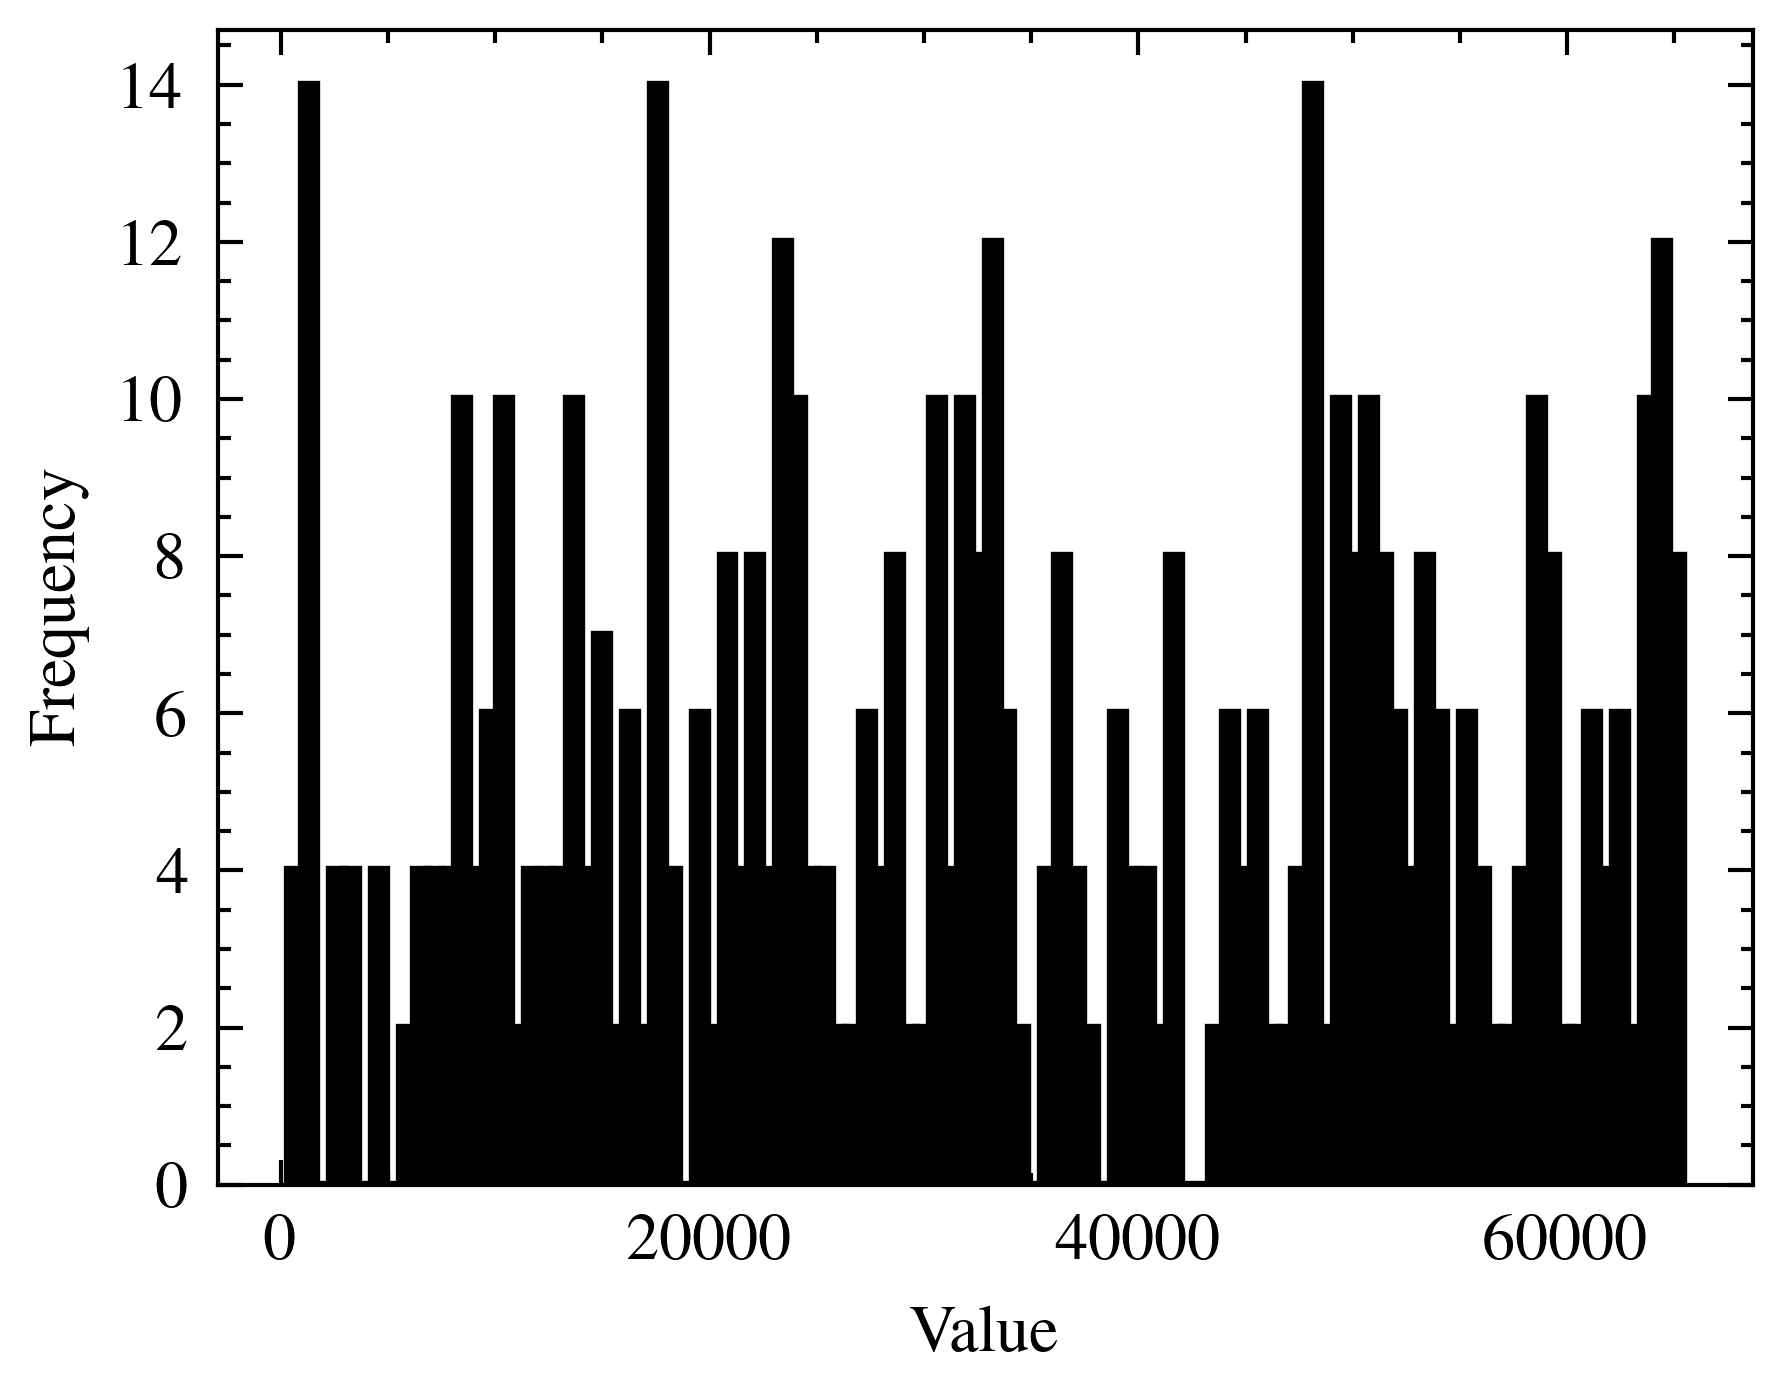
\includegraphics[width=\linewidth]{src/figures/lcg-plot/zx/lcg-2-8.png}
		\subcaption{$N=2^8$}
	\end{subfigure}
	\begin{subfigure}{0.48\linewidth}
		\centering
		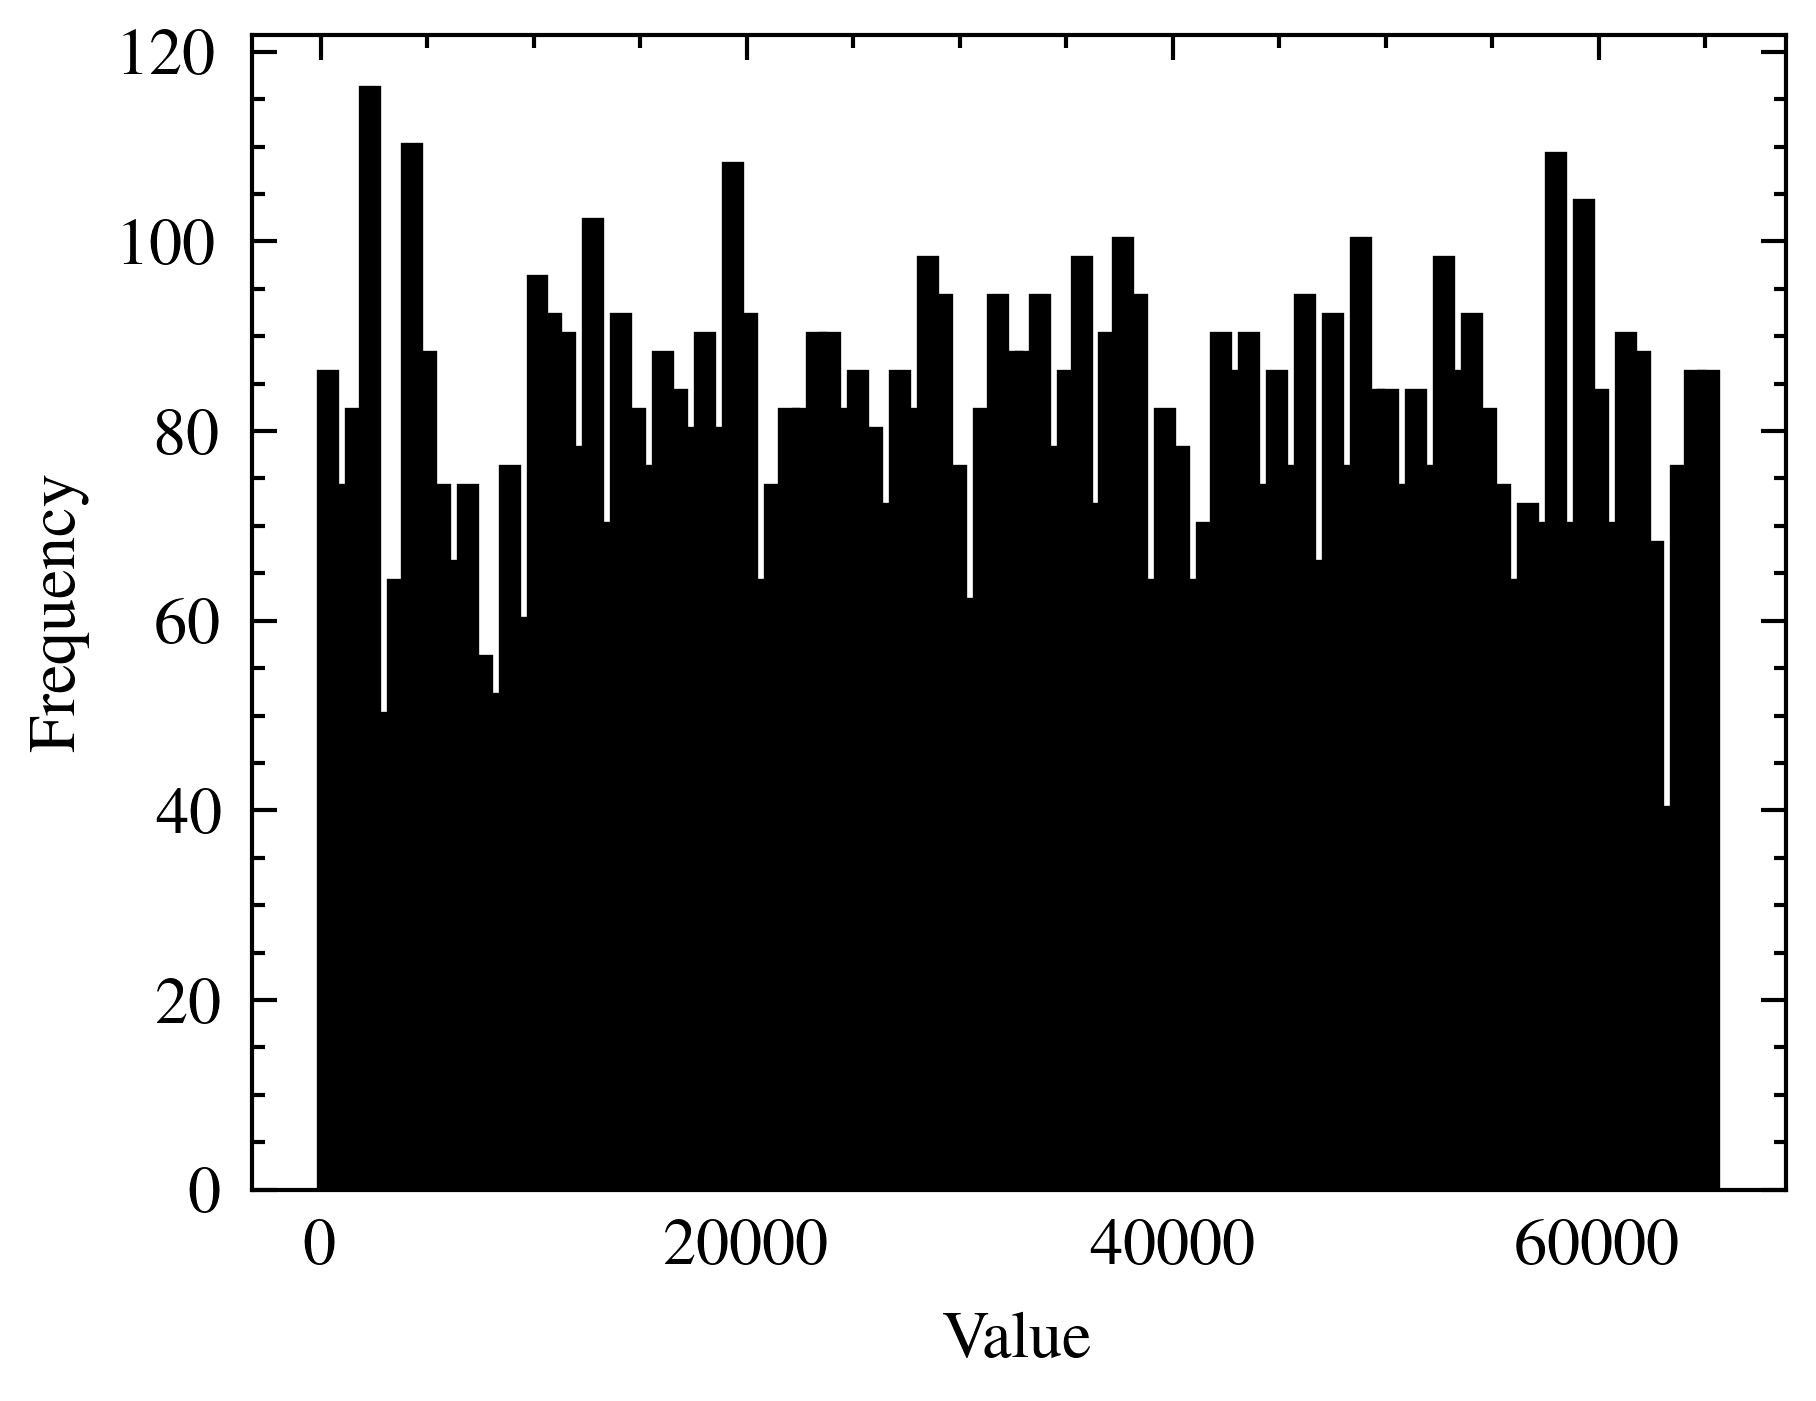
\includegraphics[width=\linewidth]{src/figures/lcg-plot/zx/lcg-2-12.png}
		\subcaption{$N=2^{12}$}
	\end{subfigure}
	\begin{subfigure}{0.48\linewidth}
		\centering
		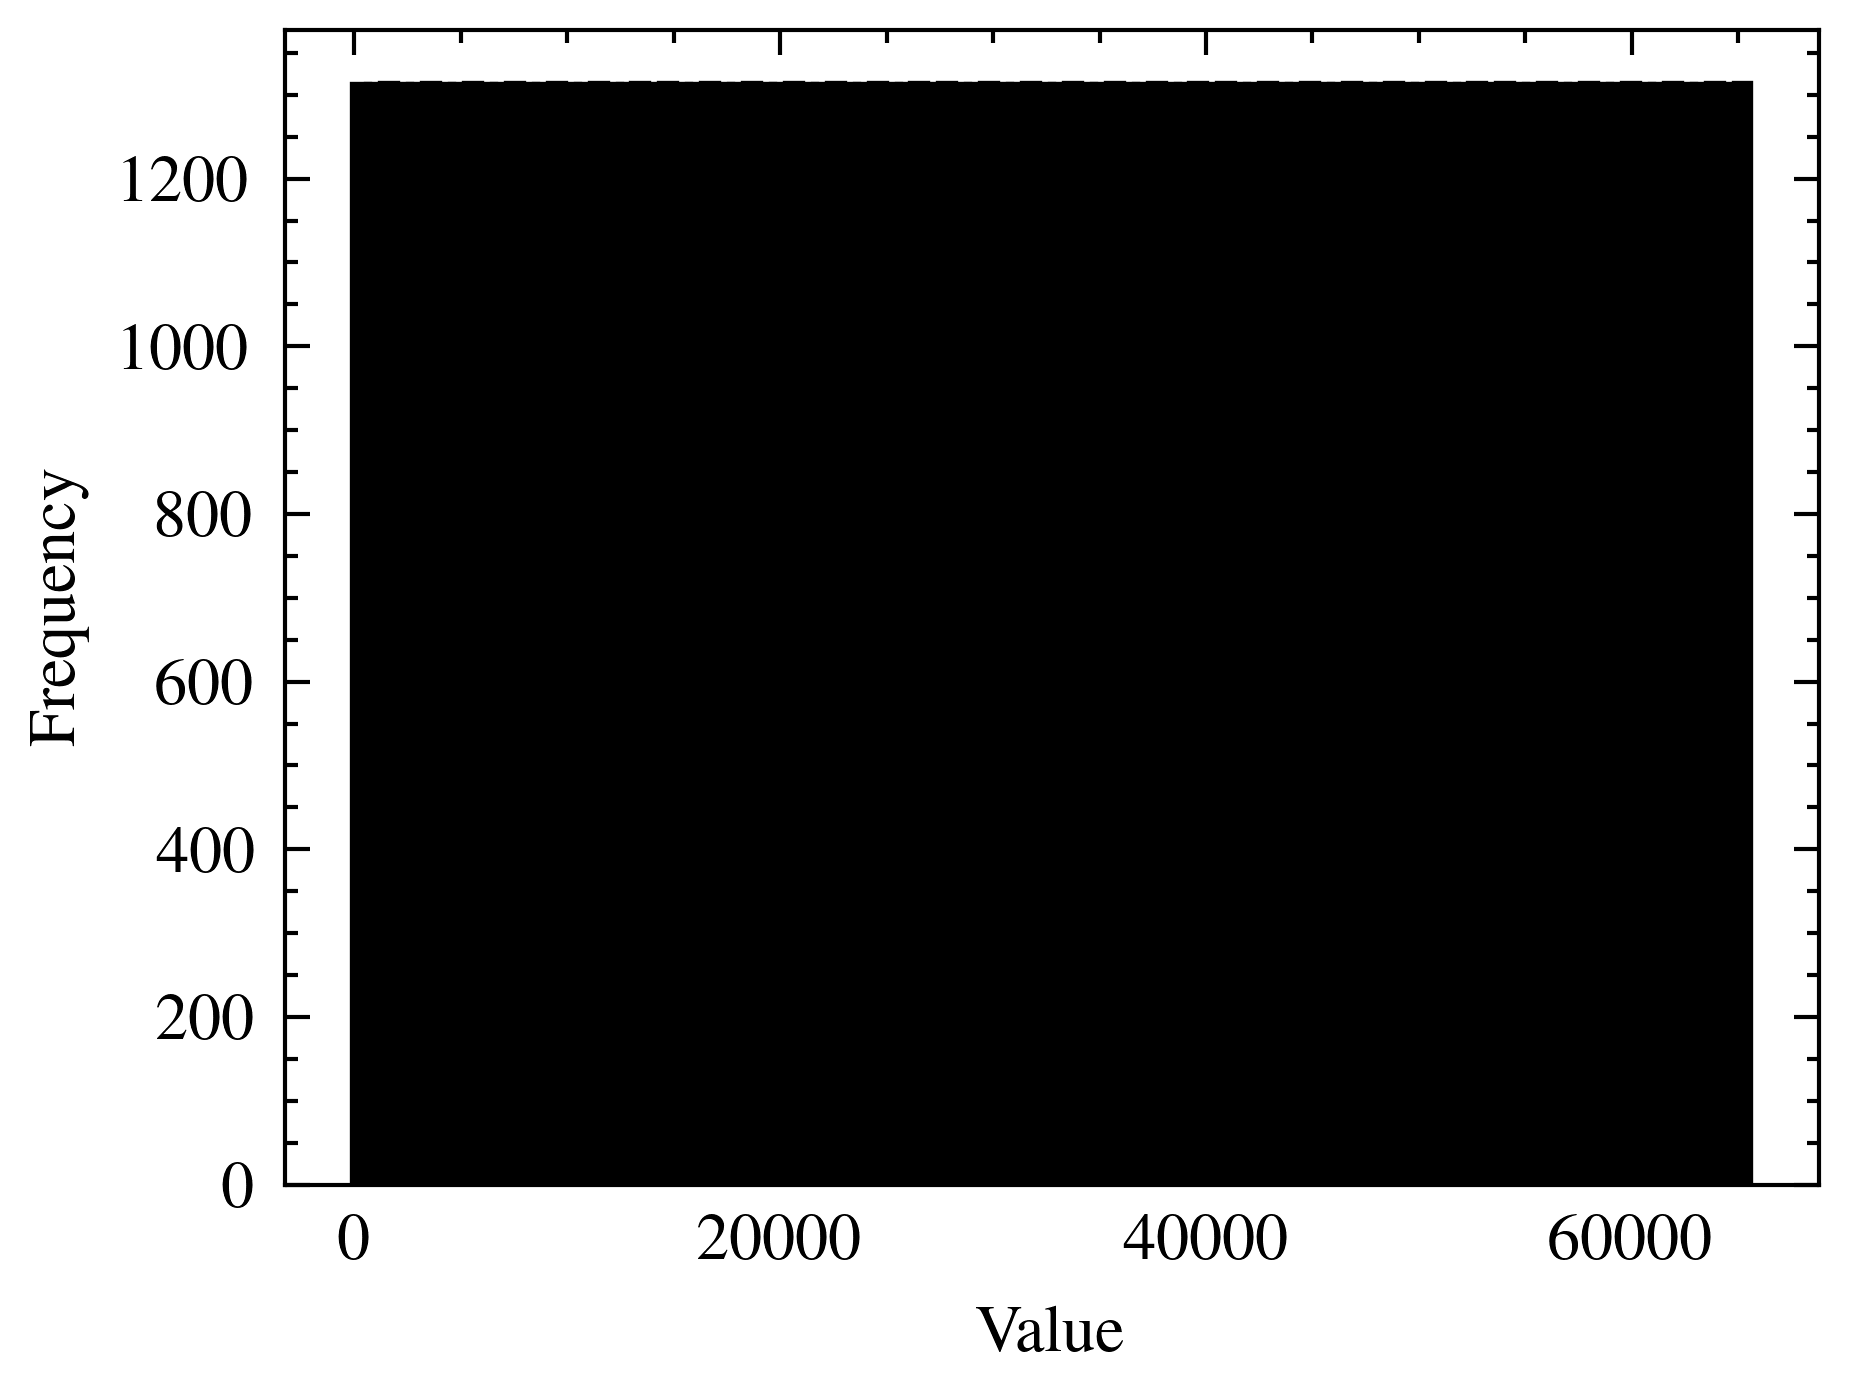
\includegraphics[width=\linewidth]{src/figures/lcg-plot/zx/lcg-2-16.png}
		\subcaption{$N=2^{16}$}
	\end{subfigure}
	\caption{線形合同法の乱数生成 $a=75, c=74, m=2^{16}+1$}\label{fig:lcg-zx}
\end{figure}

\begin{figure}
	\centering
	\begin{subfigure}{0.48\linewidth}
		\centering
		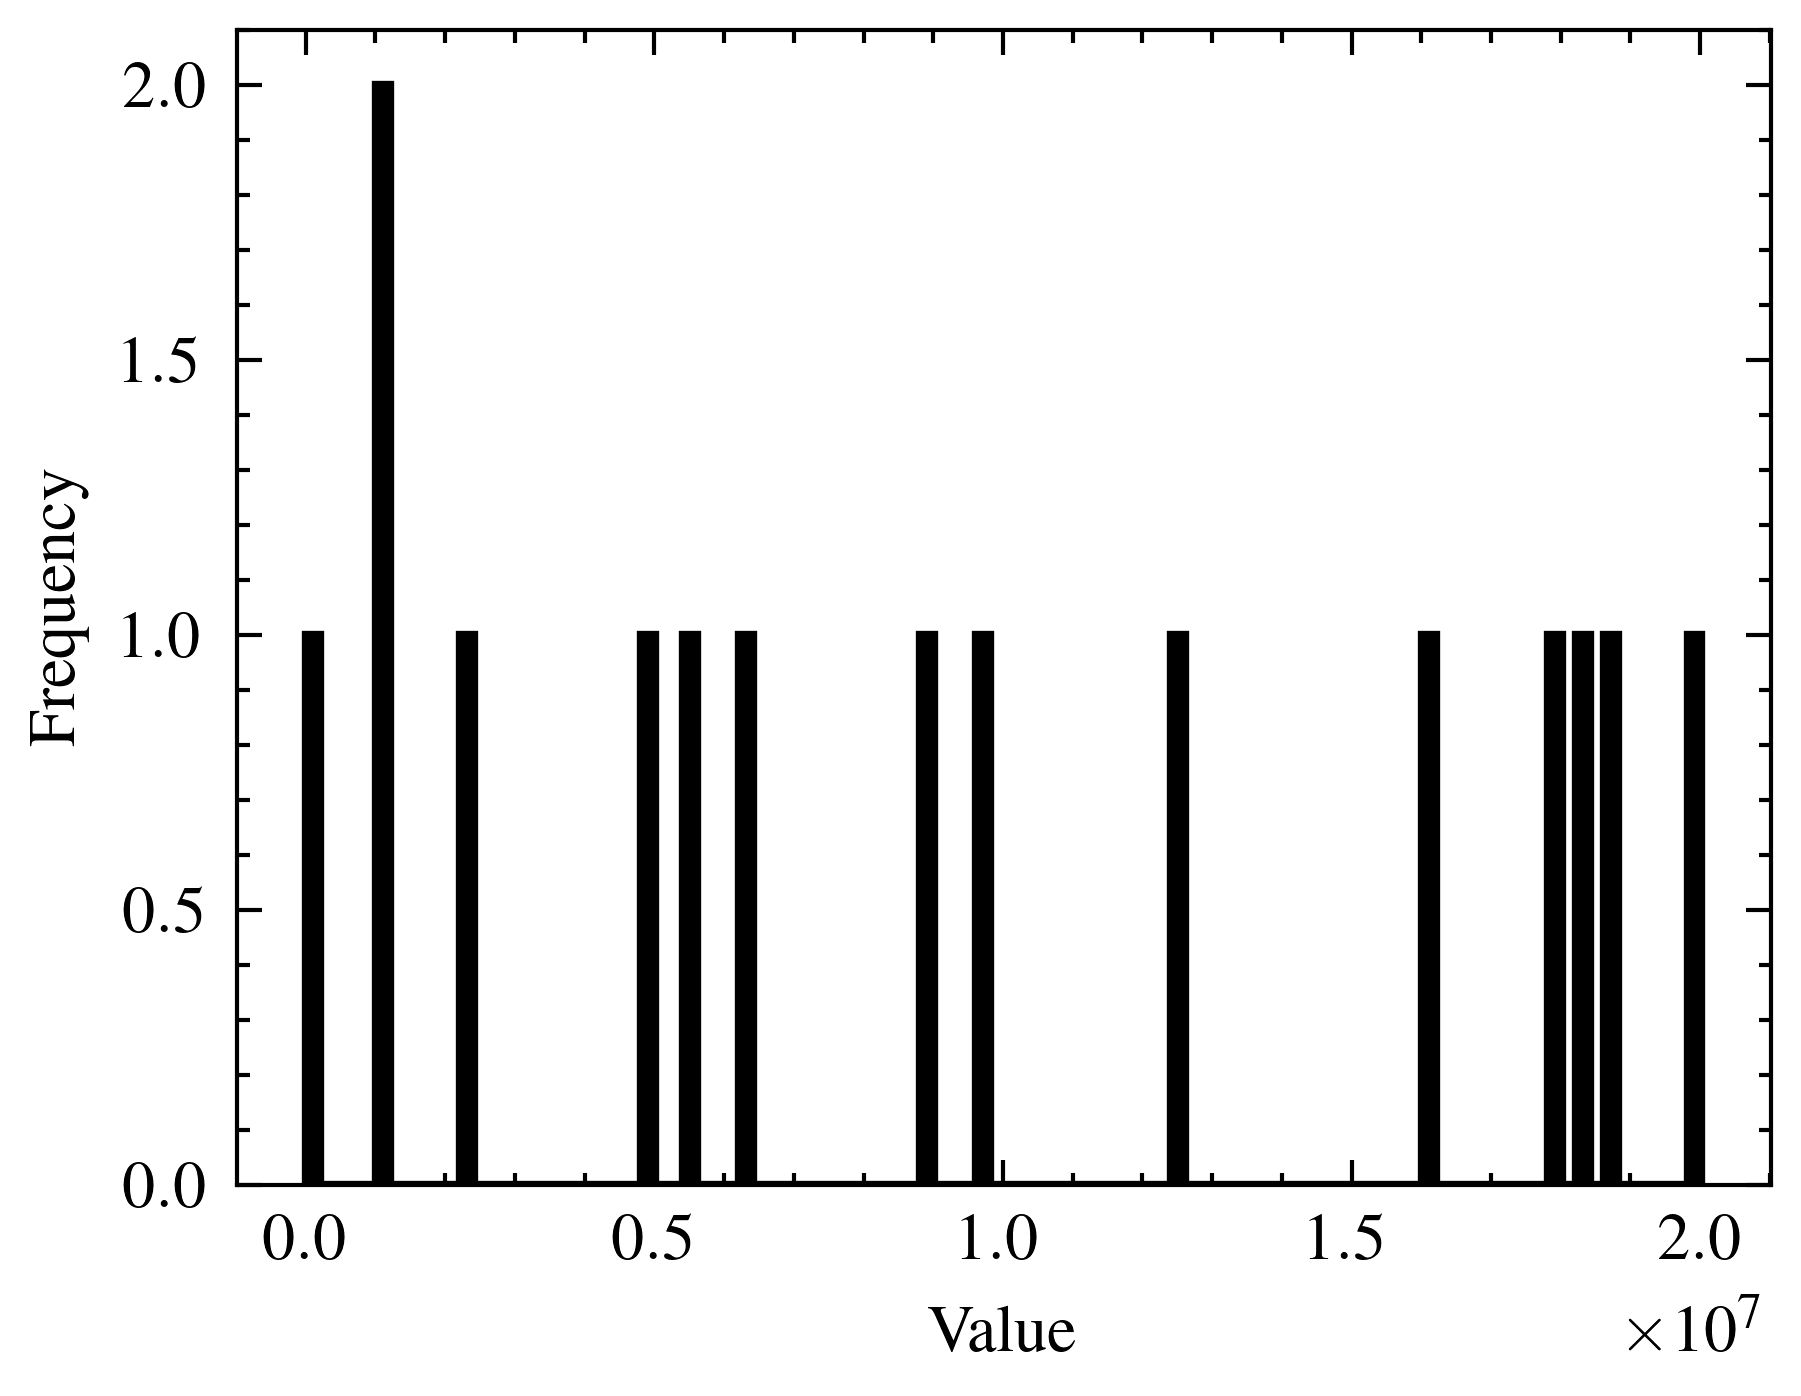
\includegraphics[width=\linewidth]{src/figures/lcg-plot/rand/lcg-2-4.png}
		\subcaption{$N=2^4$}
	\end{subfigure}
	\begin{subfigure}{0.48\linewidth}
		\centering
		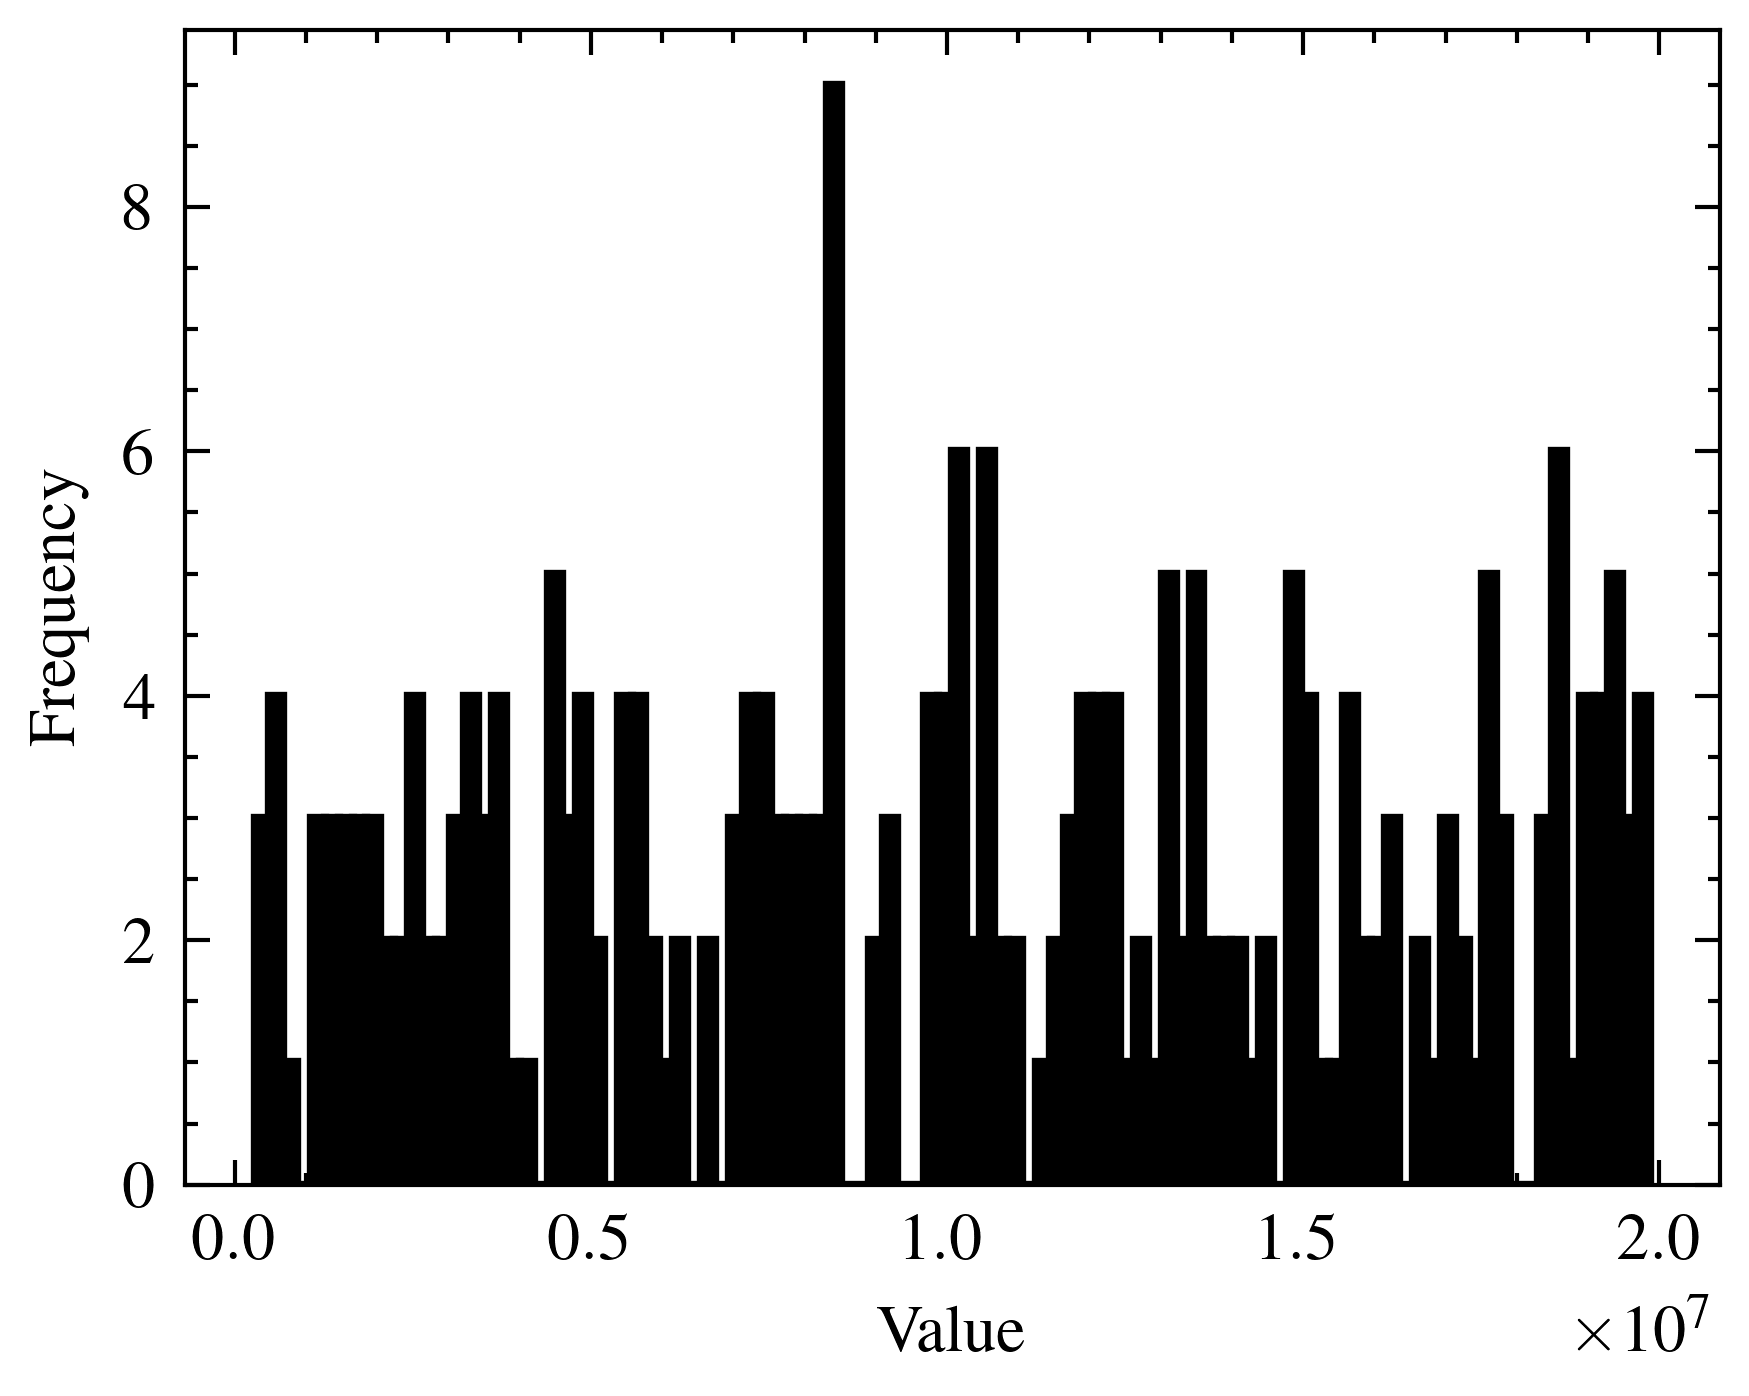
\includegraphics[width=\linewidth]{src/figures/lcg-plot/rand/lcg-2-8.png}
		\subcaption{$N=2^8$}
	\end{subfigure}
	\begin{subfigure}{0.48\linewidth}
		\centering
		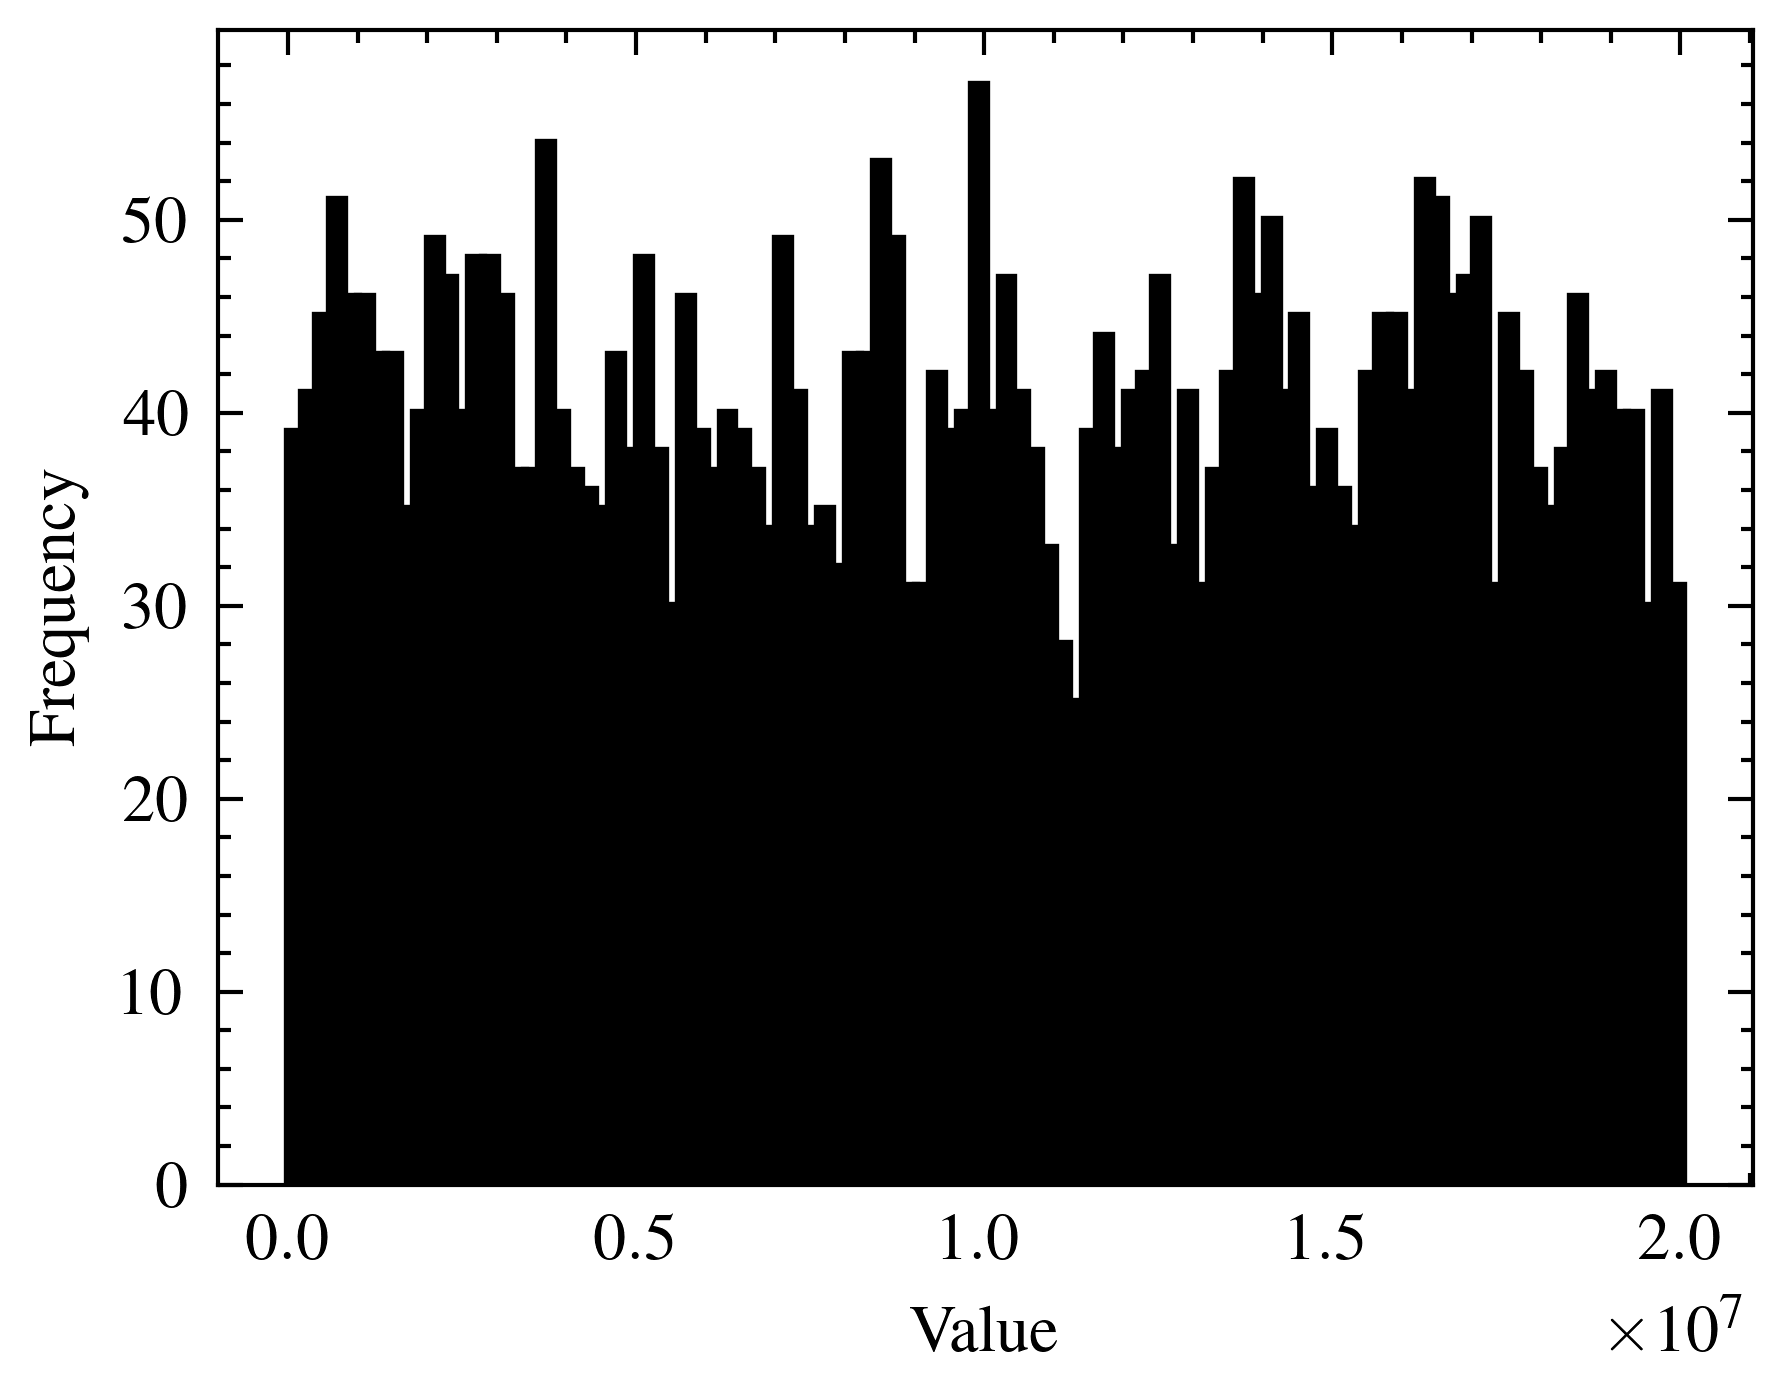
\includegraphics[width=\linewidth]{src/figures/lcg-plot/rand/lcg-2-12.png}
		\subcaption{$N=2^{12}$}
	\end{subfigure}
	\begin{subfigure}{0.48\linewidth}
		\centering
		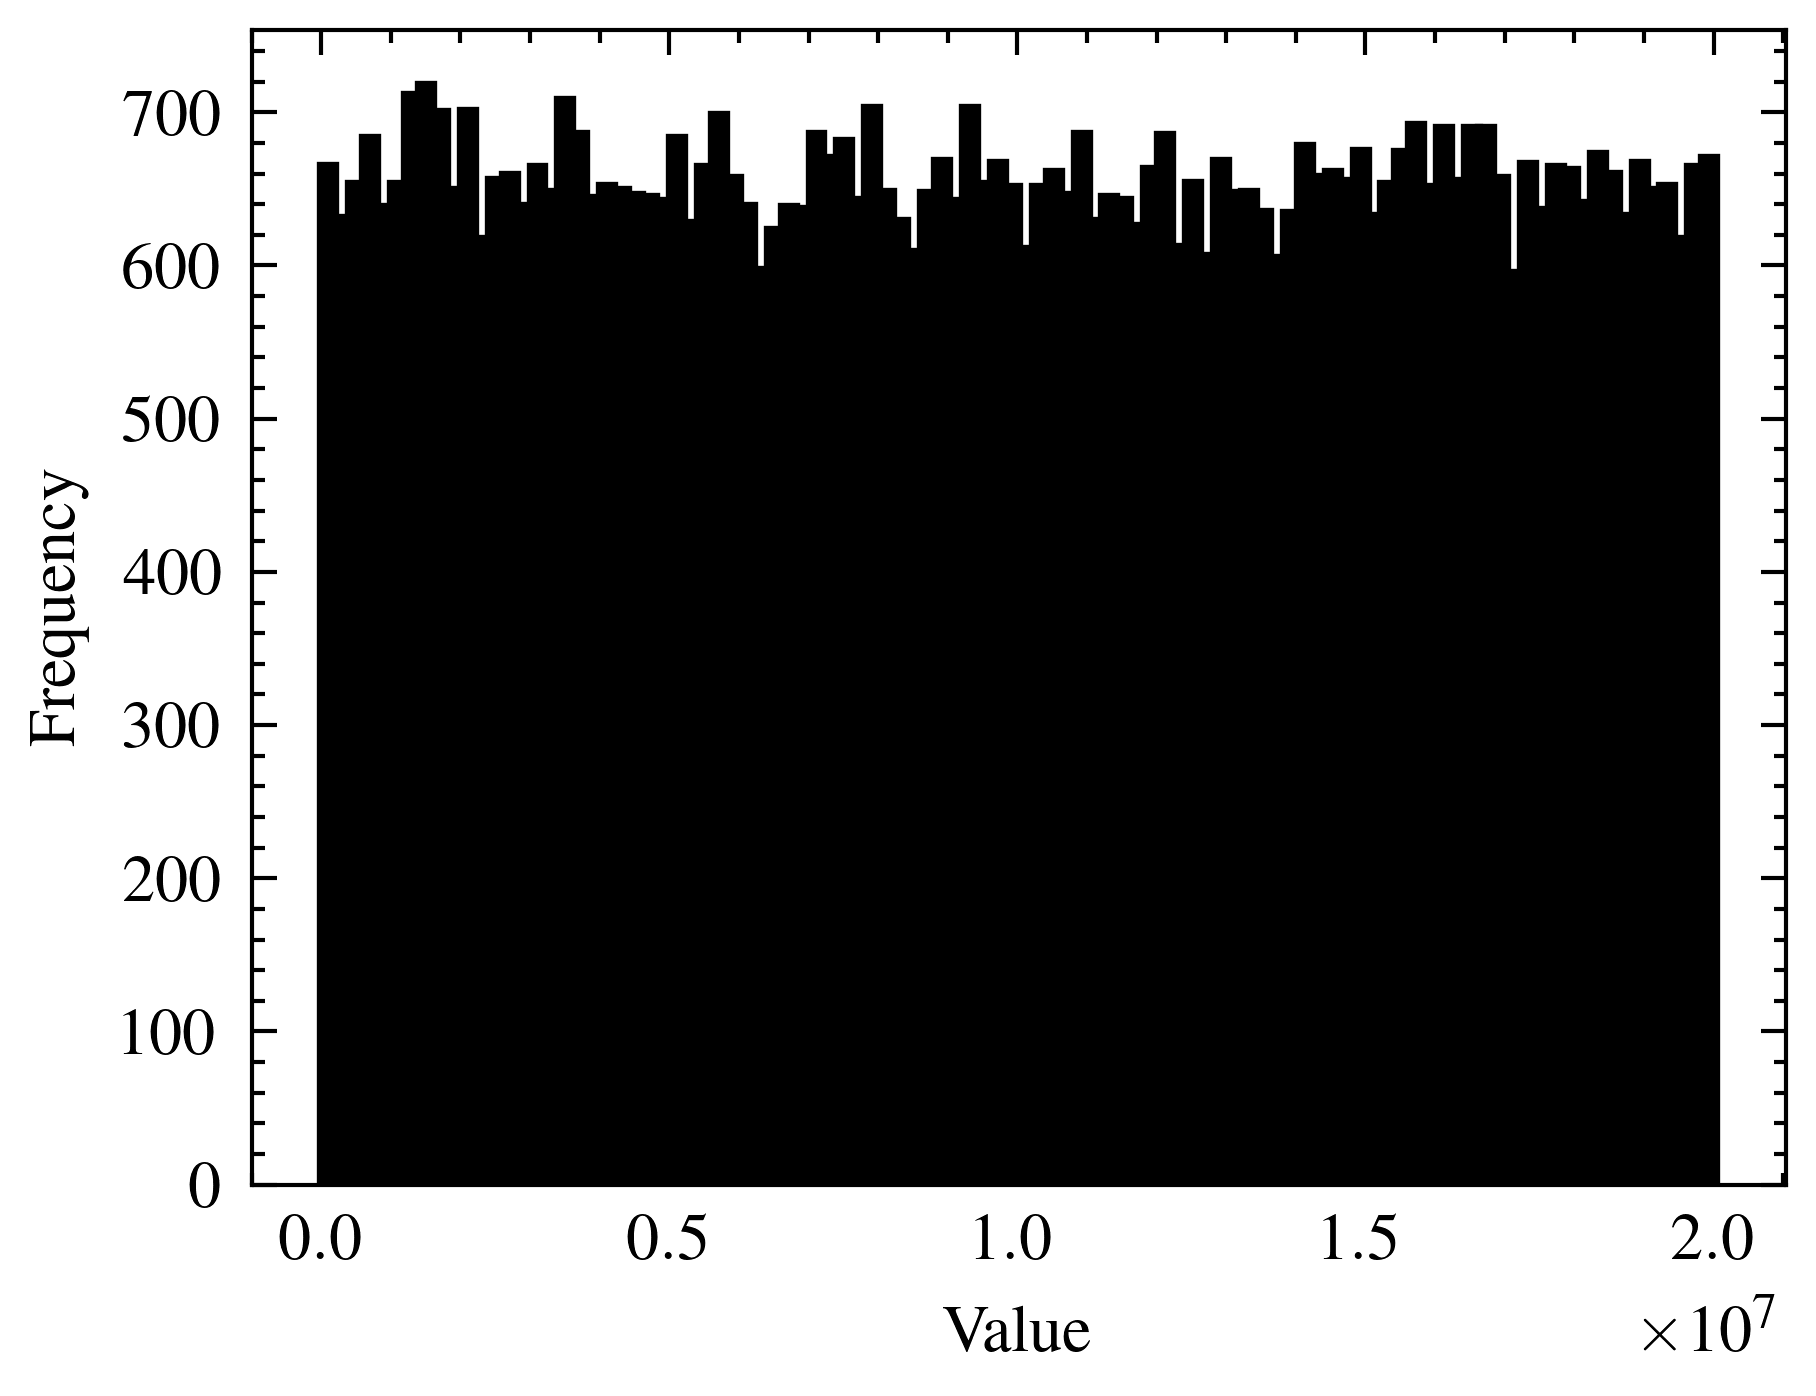
\includegraphics[width=\linewidth]{src/figures/lcg-plot/rand/lcg-2-16.png}
		\subcaption{$N=2^{16}$}
	\end{subfigure}
	\caption{線形合同法の乱数生成 $a=101, c=49, m=20040213$}\label{fig:lcg-rand}
\end{figure}


\clearpage
\subsubsection{その他乱数生成法とベンチマーク}
Go言語にて次の
\begin{itemize}
	\item math/rand pkg \footnote{
		      Go言語の標準パッケージである。
		      シードを指定することで完全に再現可能な乱数を生成することができる。
		      生成アルゴリズムはALFG(Additive Lagged Fibonacci Generator)のバリエーションとのことである。
		      現在、Go 1.22にてChaCha8を使用したmath/rand/v2が開発されている。\cite{salsa20}\cite{go-math-rand-v2}
	      }
	\item crypto/rand pkg \footnote{
		      Go言語の標準パッケージである。
		      暗号的に安全な乱数を生成することができる。
		      環境に応じたノイズをシードとして使用し、出力が予測不可能である。
	      }
	\item Middle Square Method
	\item Linear Congruential Generator
\end{itemize}
についてベンチマークを行い、それぞれの特性や性能を比較する。
なお、LCGのパラメータは$m=2^{16} + 1$, $a=75$, $c=74$とした。\footnote{
	ZX81と呼ばれるコンピュータにて使われているパラメータである。
}
3秒間のベンチマークを行った結果を表\ref{tab:random-bench}に示す。
LCGが最もメモリ消費量が少なく、最も高速であることがわかる。
MSMはメモリ消費量、速度ともにLCGより劣る。
MSMが遅い理由としては、Go言語においてある数から中央の部分を取り出す処理が遅いということが考えられる。
math/randの場合は、LCGよりは遅く、メモリ消費量も少ない。
crypto/randは、メモリ消費量が最も多く、速度もLCGより遅い。
これは暗号学的に安全な乱数を生成するために、より多くの計算を行うためである。

\paragraph{Middle Square Method (MSM)}
平方菜中法は、乱数生成アルゴリズムの一つである。
乱数生成アルゴリズムの中でも最も単純なものの一つであり、
乱数のシードを2乗し、その中央の部分を取り出すことで乱数を生成する。

\begin{longtable}{|c|c|c|c|}
	\caption{乱数生成法のベンチマーク}\label{tab:random-bench}    \\
	\hline
	生成法         & 生成数       & 時間 / ns/op & メモリ / B/op \\
	\hline
	\endfirsthead

	\hline
	生成法         & 生成数       & 時間 / ns/op & メモリ / B/op \\
	\hline
	\endhead

	\hline
	\endfoot

	\hline
	\endlastfoot

	math/rand   & 384210751 & 9.342      & 0          \\
	crypto/rand & 6548737   & 554.5      & 56         \\
	lcg         & 565856049 & 6.321      & 0          \\
	msm         & 39674995  & 84.90      & 16         \\
\end{longtable}


\subsubsection{疑似乱数の活用}
擬似乱数法の応用、特に暗号学的擬似乱数についてまとめる。
暗号学的擬似乱数とは、乱数生成法と出力が既知である場合にも出力が予測できないような乱数生成法のことである。
代表的な方法としては、暗号学的ハッシュ関数と呼ばれる一方向性の関数を使用する方法である。
暗号学的ハッシュ関数には、
\begin{itemize}
	\item 原像計算困難性
	      ハッシュ値からもとのメッセージを計算することが困難であること
	\item 強衝突耐性
	      ある2つ以上のメッセージから同じハッシュが得られることが事実上不可能であること
\end{itemize}
といった性質が求められる。
代表的な生成法は、
\begin{itemize}
	\item SHA-1
	\item SHA-256
	\item MD-5
\end{itemize}
などがあげられる。
SHA-1は、2017年にGoogleがSHA-1の衝突を発見した。\cite{google-sha1-collision}
そのため今では使用が推奨されていない。
これらの関数は、例えばパスワードのハッシュ化や、ファイル・DockerイメージなどのChecksum、暗号通貨などに使用される。
パスワードでは原像計算困難性が大事である。
Checksumでは強衝突耐性と、すなわちハッシュが一致すればファイルが一致することが保証されることが重要である。
暗号通貨では、強衝突耐性とこれらハッシュ関数に必要な計算量、加えて情報の圧縮などが重要な役割を果たす。

\subsubsection{乱数によるブラウン運動のシミュレーション}
ブラウン運動とは、溶媒中の微粒子が溶媒分子の衝突によってランダムに運動する現象である。
ブラウン運動は次の
\begin{equation}\label{eq:brownian-motion}
	\odv{\bm{v}}{t} = \alpha \bm{v} + \bm{f}
\end{equation}
という運動方程式で表すことができる。
これを差分方程式化すると、
\begin{equation}
	\bm{v}_{t+1} = \left(1 - \dfrac{\alpha \Delta t}{m}\right) \bm{v}_t + \dfrac{\bm{f} \Delta t}{m}
\end{equation}
となり、漸化式を得る。
粒子は巨視的に見れば動かないことから平均速度が0と期待されること、
$f$が同一の分布に従うことなどから、
$\bm{v}$の分散は
\begin{equation}
	\ev{(v - \ev{v})^2} = \dfrac{\Delta t}{2 \alpha m} \ev{(f - \ev{f})^2}
\end{equation}
と書け、また気体分子運動論から$\ev{v^2} = \dfrac{kT}{m}$であることを考慮すると、
\begin{equation}
	\ev{(f - \ev{f})^2} = \dfrac{2 \alpha k T}{\Delta t}
\end{equation}
となる。
よって、平均0、分散が$\dfrac{2 \alpha k T}{\Delta t}$の正規分布に従う乱数を用いることで、\footnote{
	結局、$v$を正規分布に従う乱数で更新してもよく、
	\begin{equation}
		x_{t+1} = x_t + \mathcal{N}
	\end{equation}
	としてもよい。
	この場合は、オーダーに注意である。
}
$v$を計算し、
\begin{equation}
	\bm{r}_{t+1} = \bm{r}_t + \bm{v} \Delta t
\end{equation}
で位置を更新すれば、ブラウン運動をシミュレーションすることができる。\footnote{
	詳しくは\cite{brownian-motion-report}課題8を参照
}

実際に、この方法でブラウン運動をシミュレーションし、その結果を図\ref{fig:brownian-2d-sim}に示す。
\begin{figure}
	\centering
	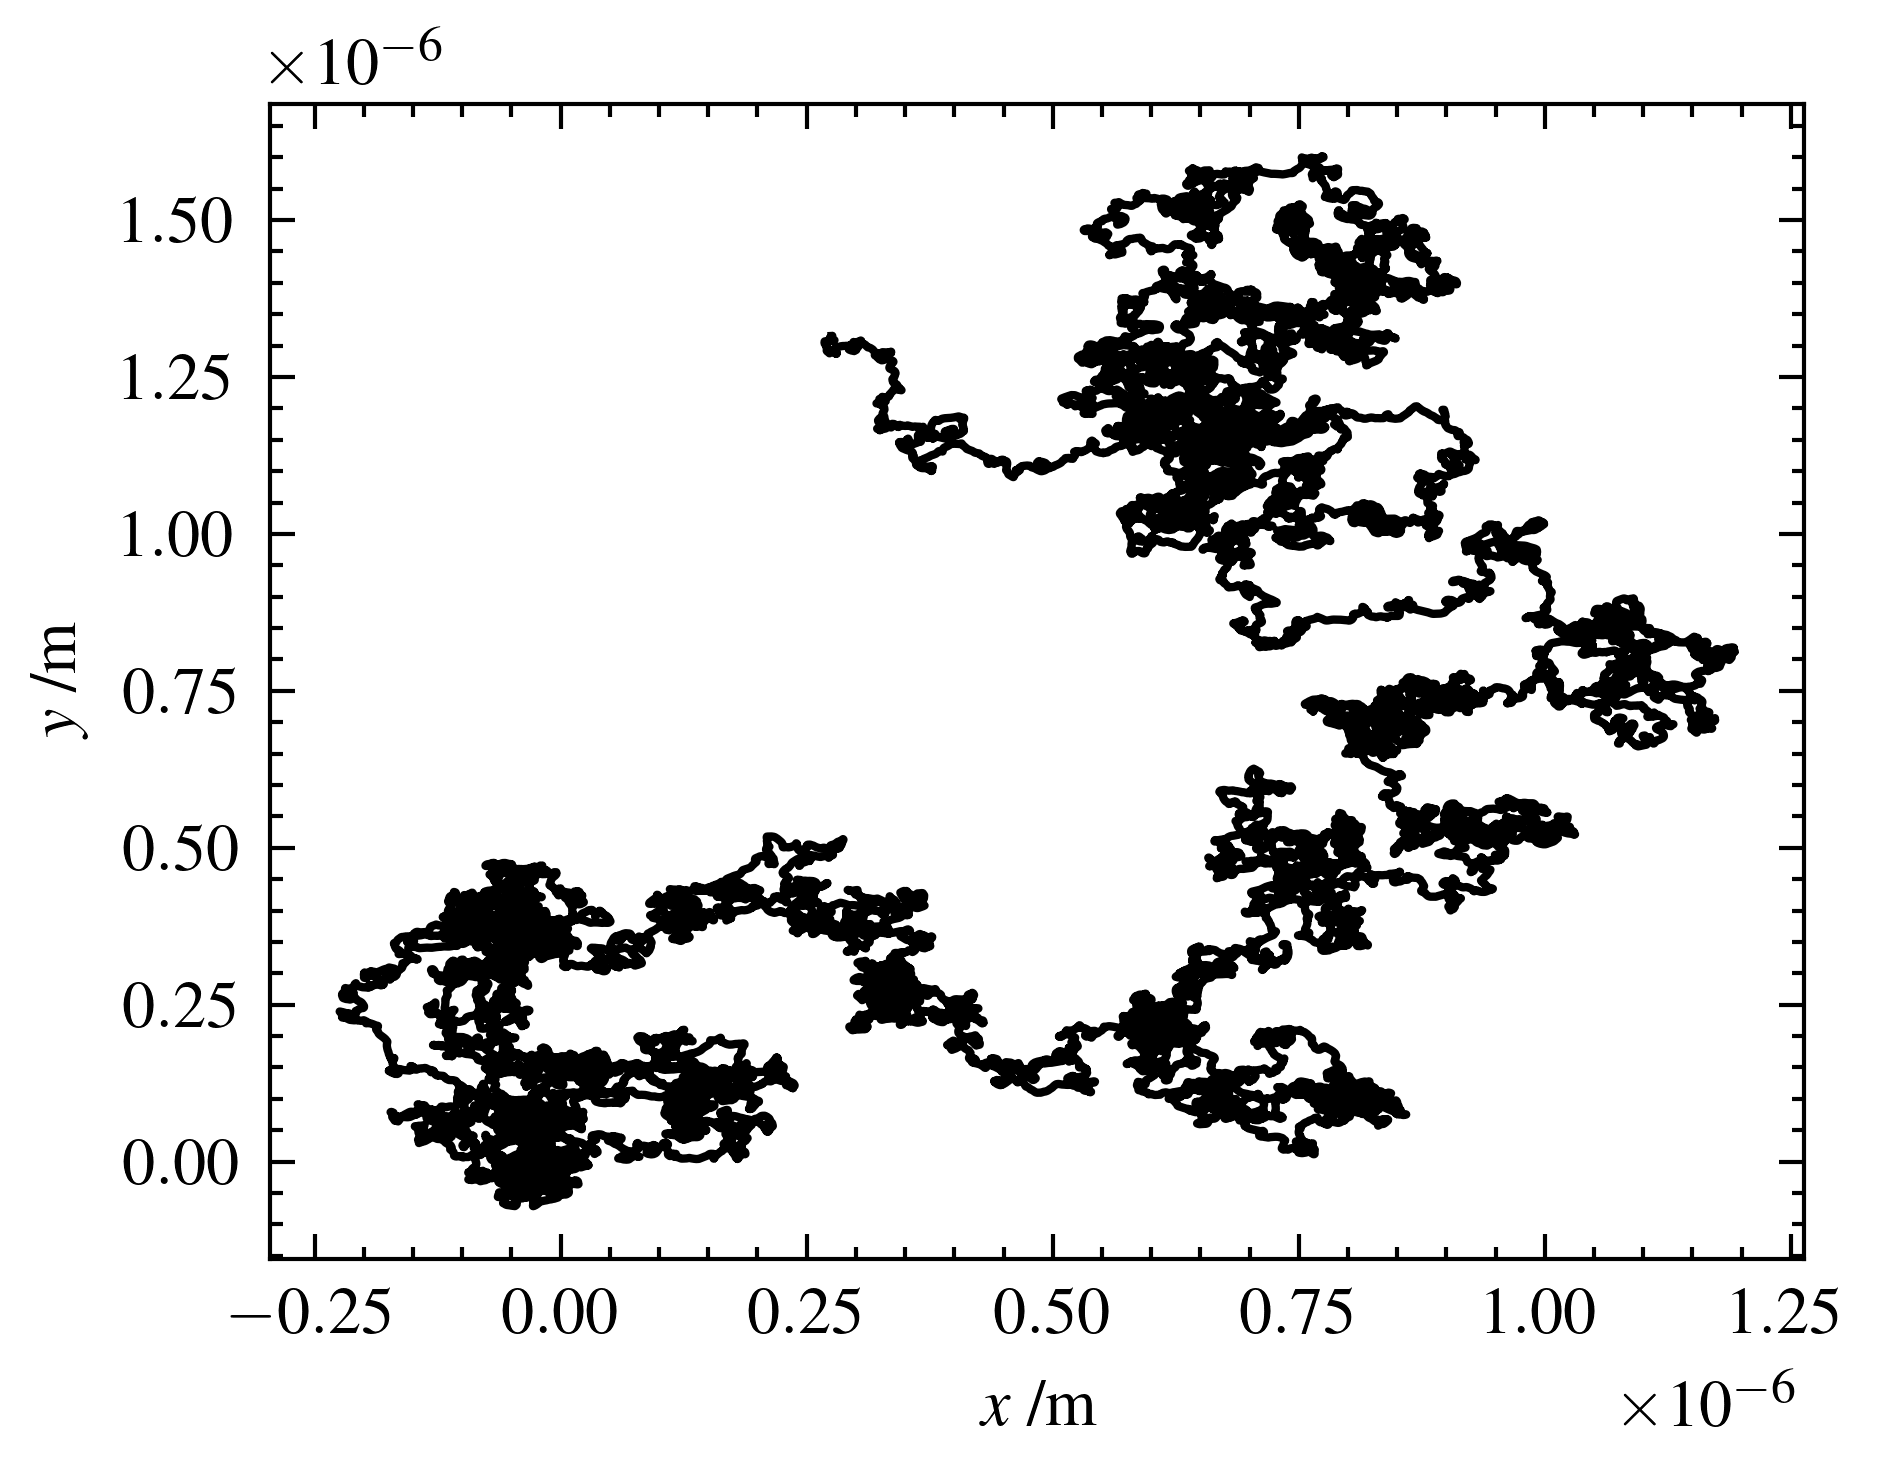
\includegraphics[width=0.8\linewidth]{./src/figures/brownian-2d-sim/brownian-2d-sim.png}
	\caption{2次元ブラウン運動のシミュレーション}\label{fig:brownian-2d-sim}
\end{figure}



\subsection{重回帰分析}

\subsubsection{実験における重回帰分析の改良}
実験では一次関数を用いて重回帰分析を行った。
より次数を上げた多項式回帰を行うことで、より適切なモデルを構築することができる。
$n$を1から4まで変化させたときの多項式回帰の結果を図\ref{fig:polynomial-regression}に示す。
\begin{figure}
    \centering
    \begin{subfigure}{0.48\linewidth}
        \centering
        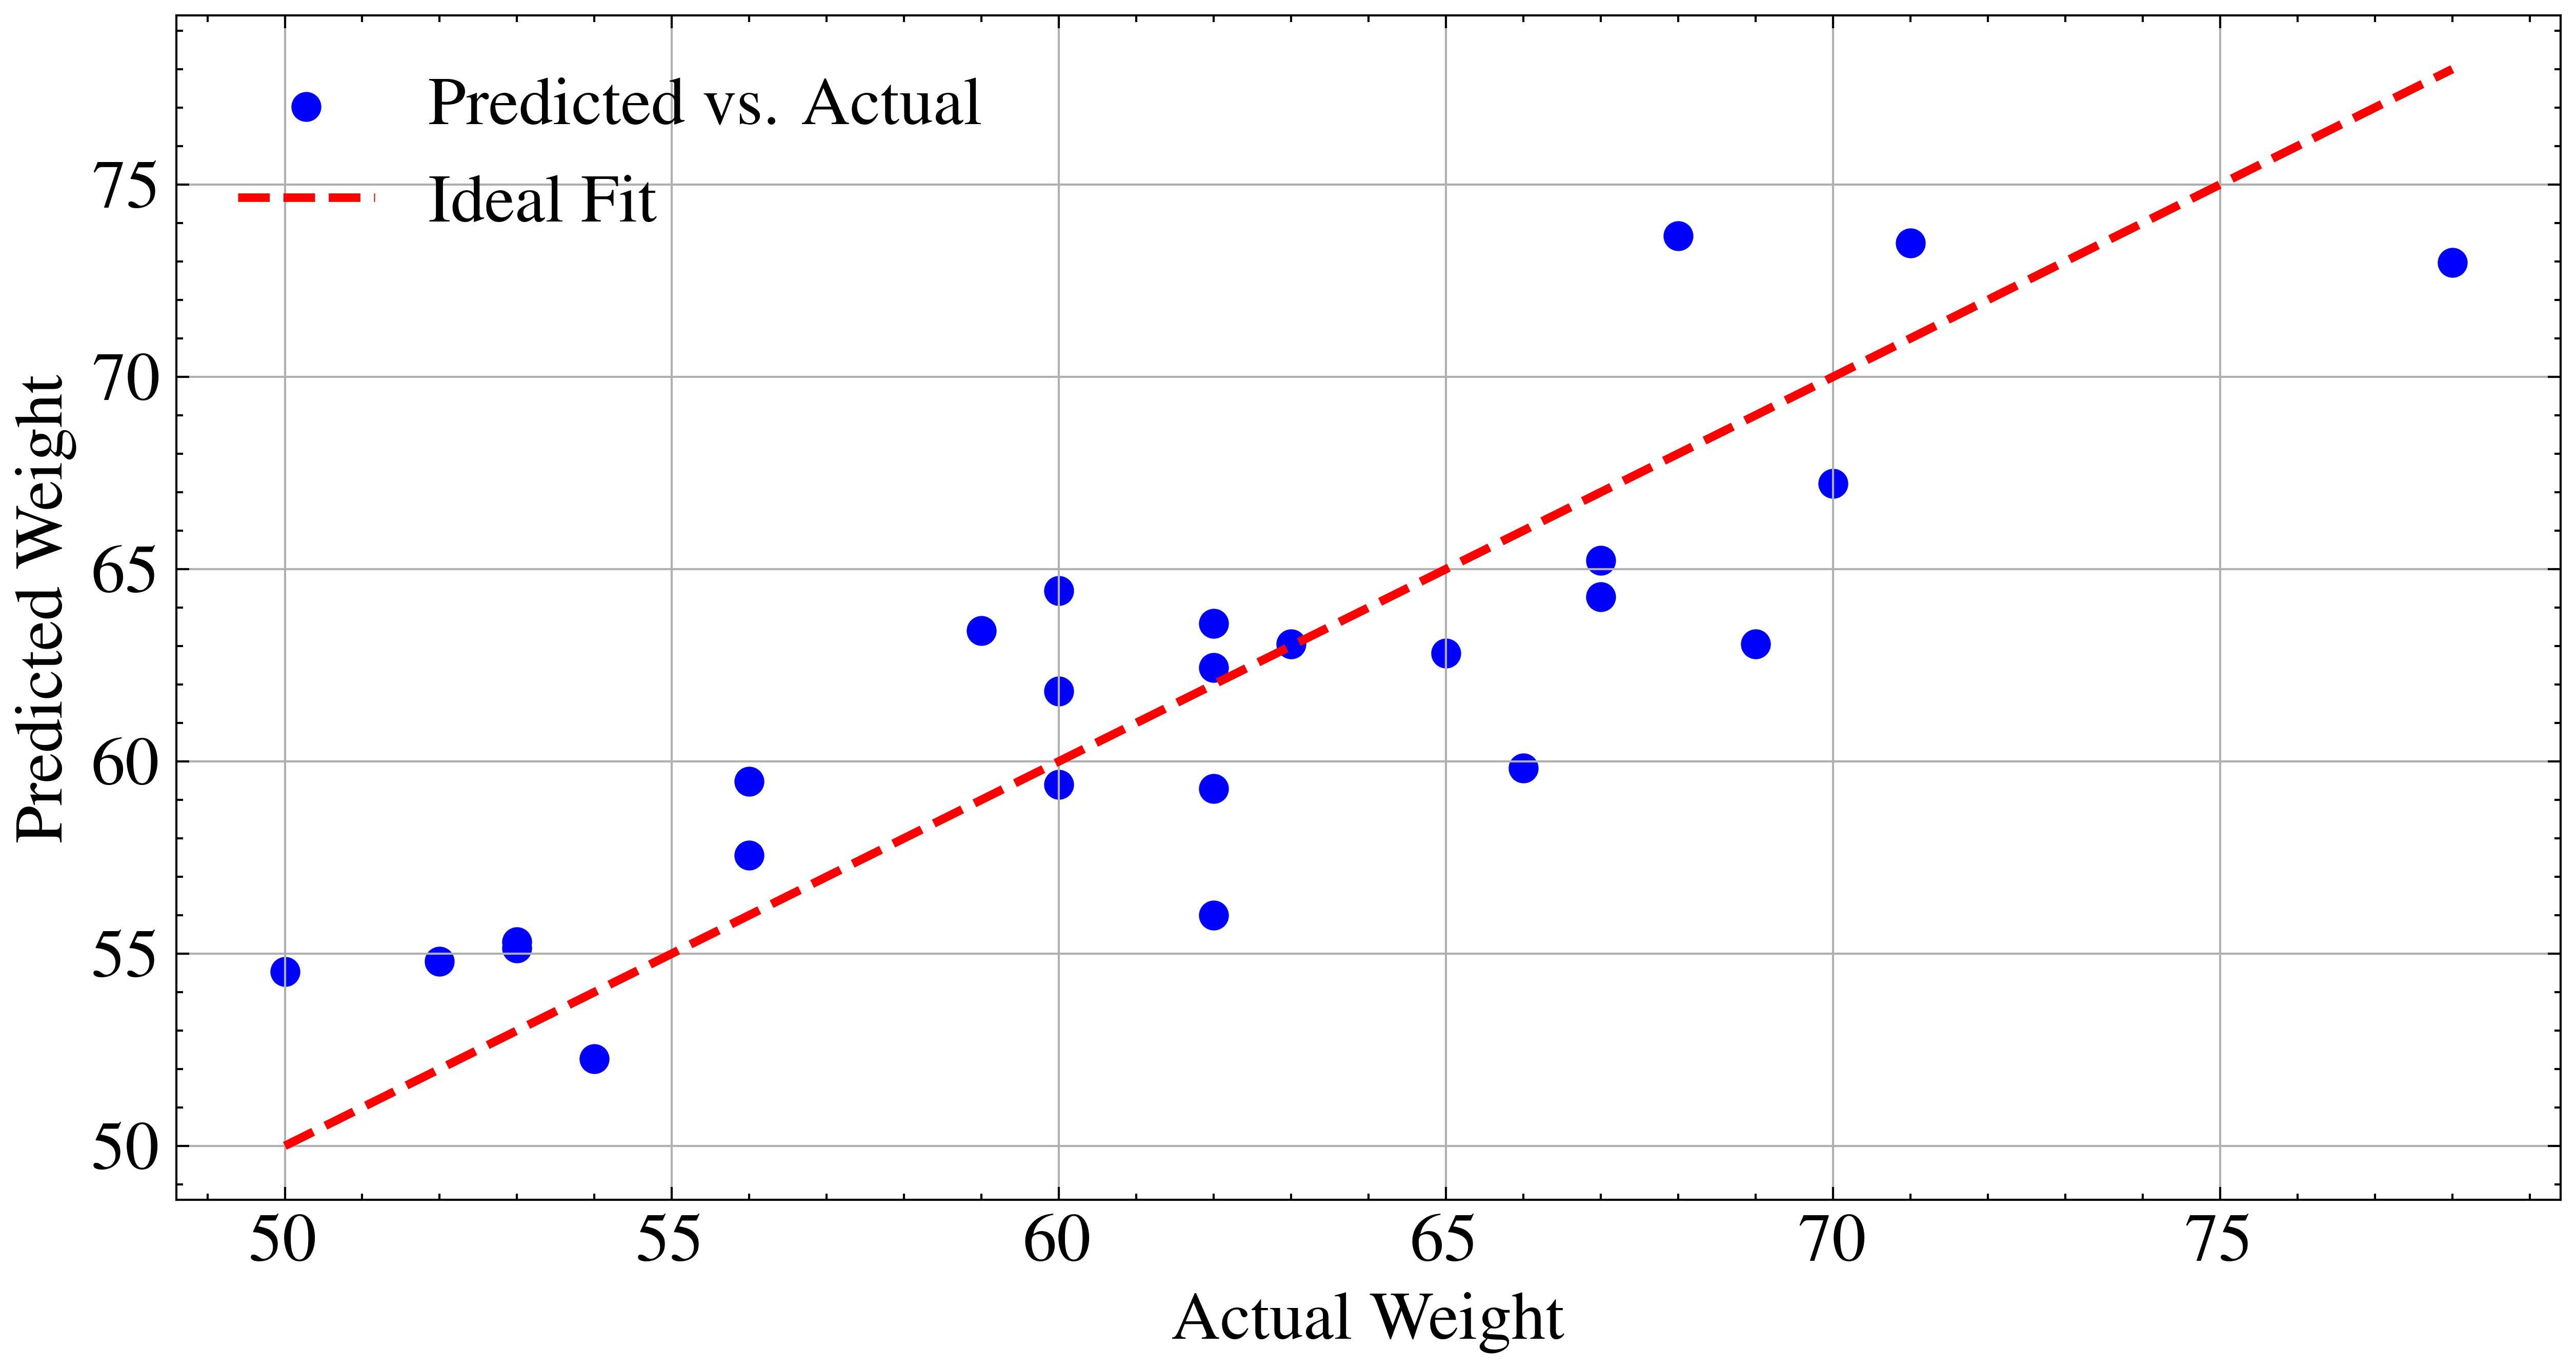
\includegraphics[width=\linewidth]{src/figures/polynominal-regression/polynomial_regression-n-1.png}
        \subcaption{$n=1$}
    \end{subfigure}
    \begin{subfigure}{0.48\linewidth}
        \centering
        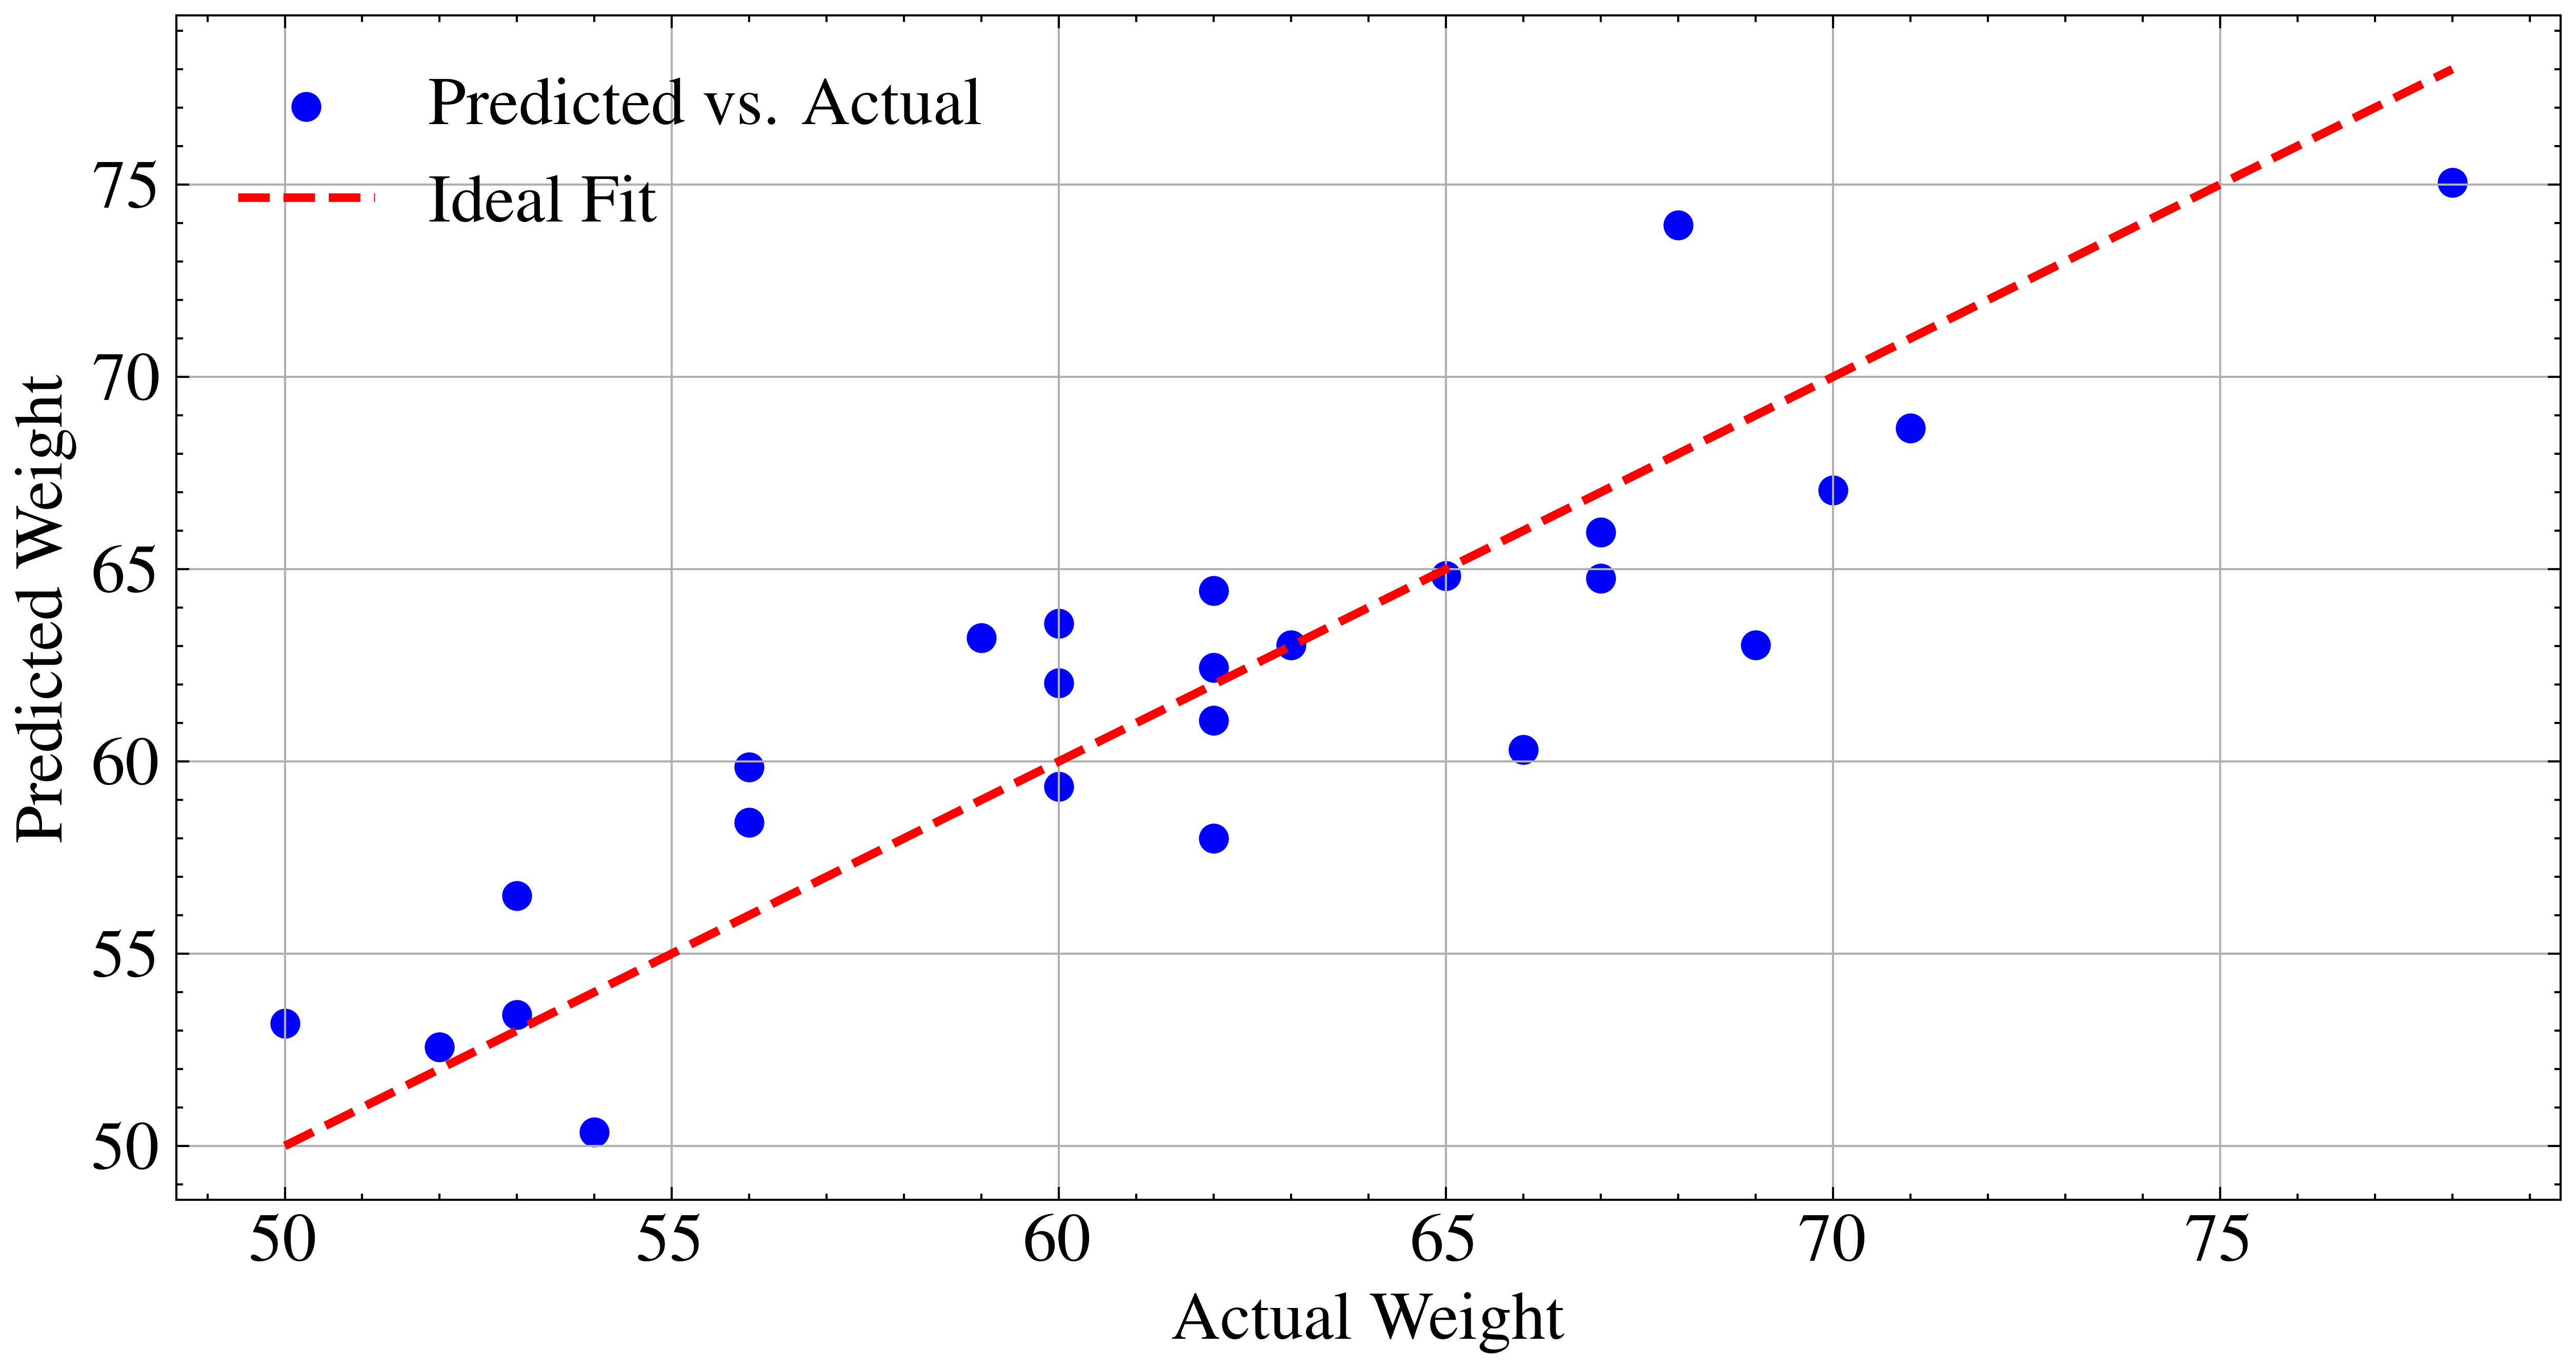
\includegraphics[width=\linewidth]{src/figures/polynominal-regression/polynomial_regression-n-2.png}
        \subcaption{$n=2$}
    \end{subfigure}
    \begin{subfigure}{0.48\linewidth}
        \centering
        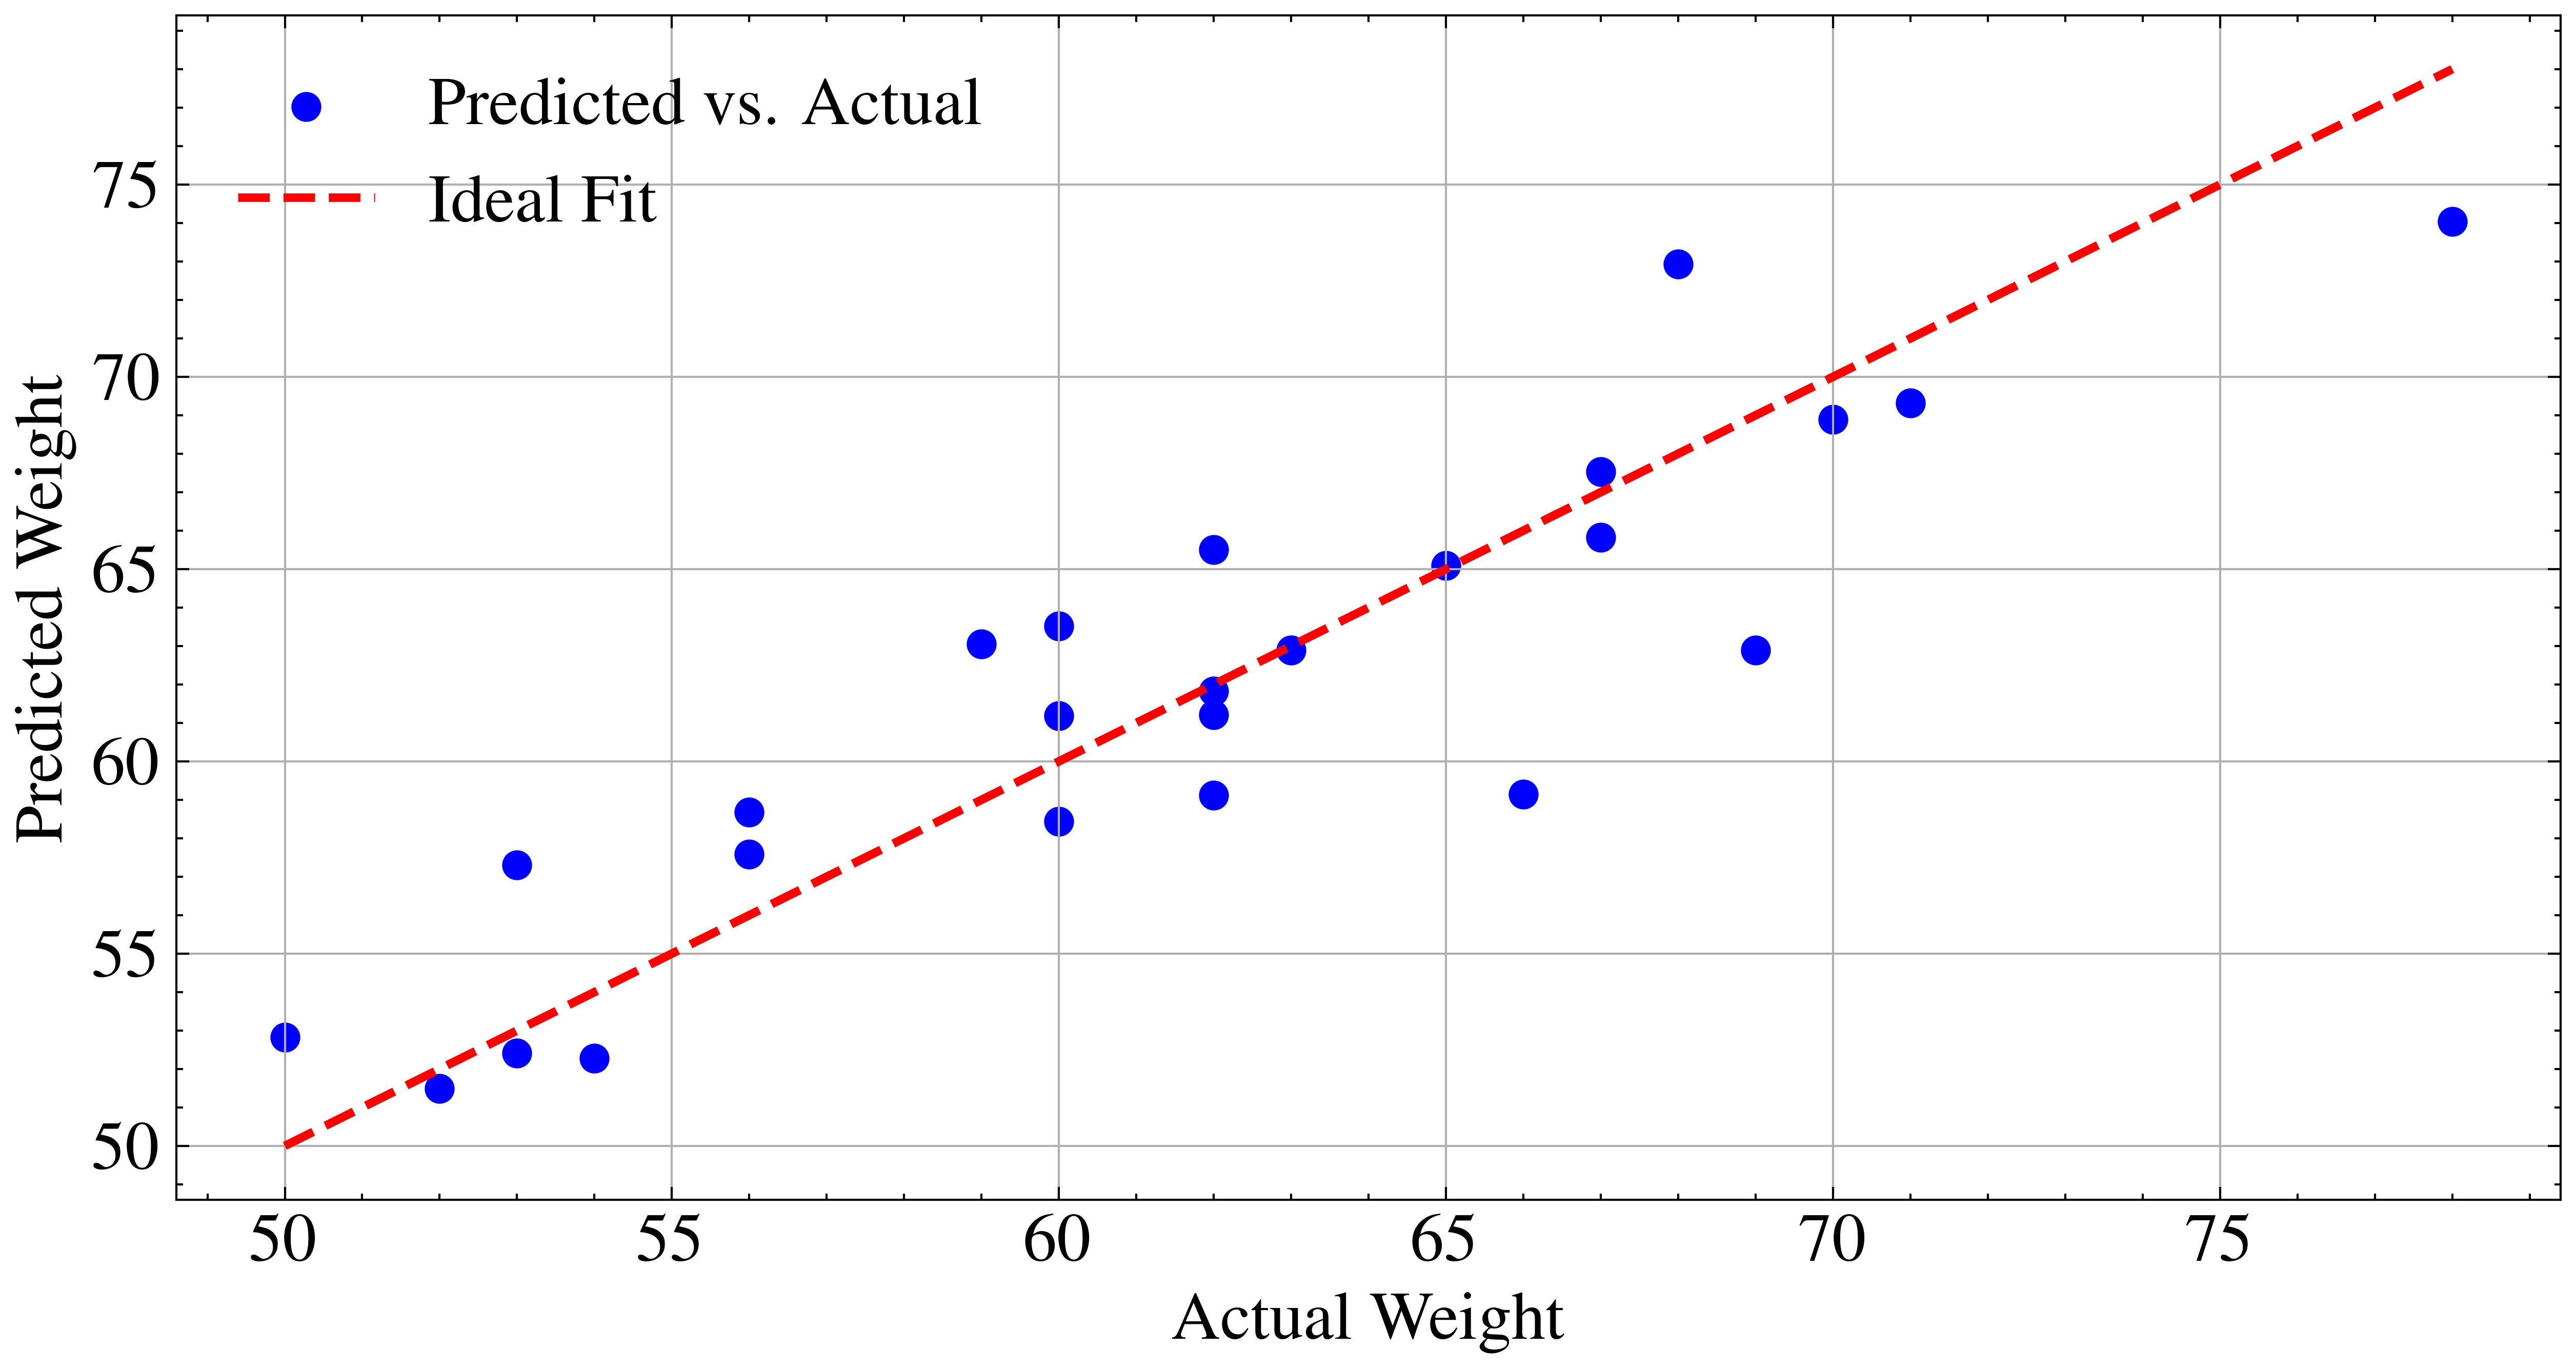
\includegraphics[width=\linewidth]{src/figures/polynominal-regression/polynomial_regression-n-3.png}
        \subcaption{$n=3$}
    \end{subfigure}
    \begin{subfigure}{0.48\linewidth}
        \centering
        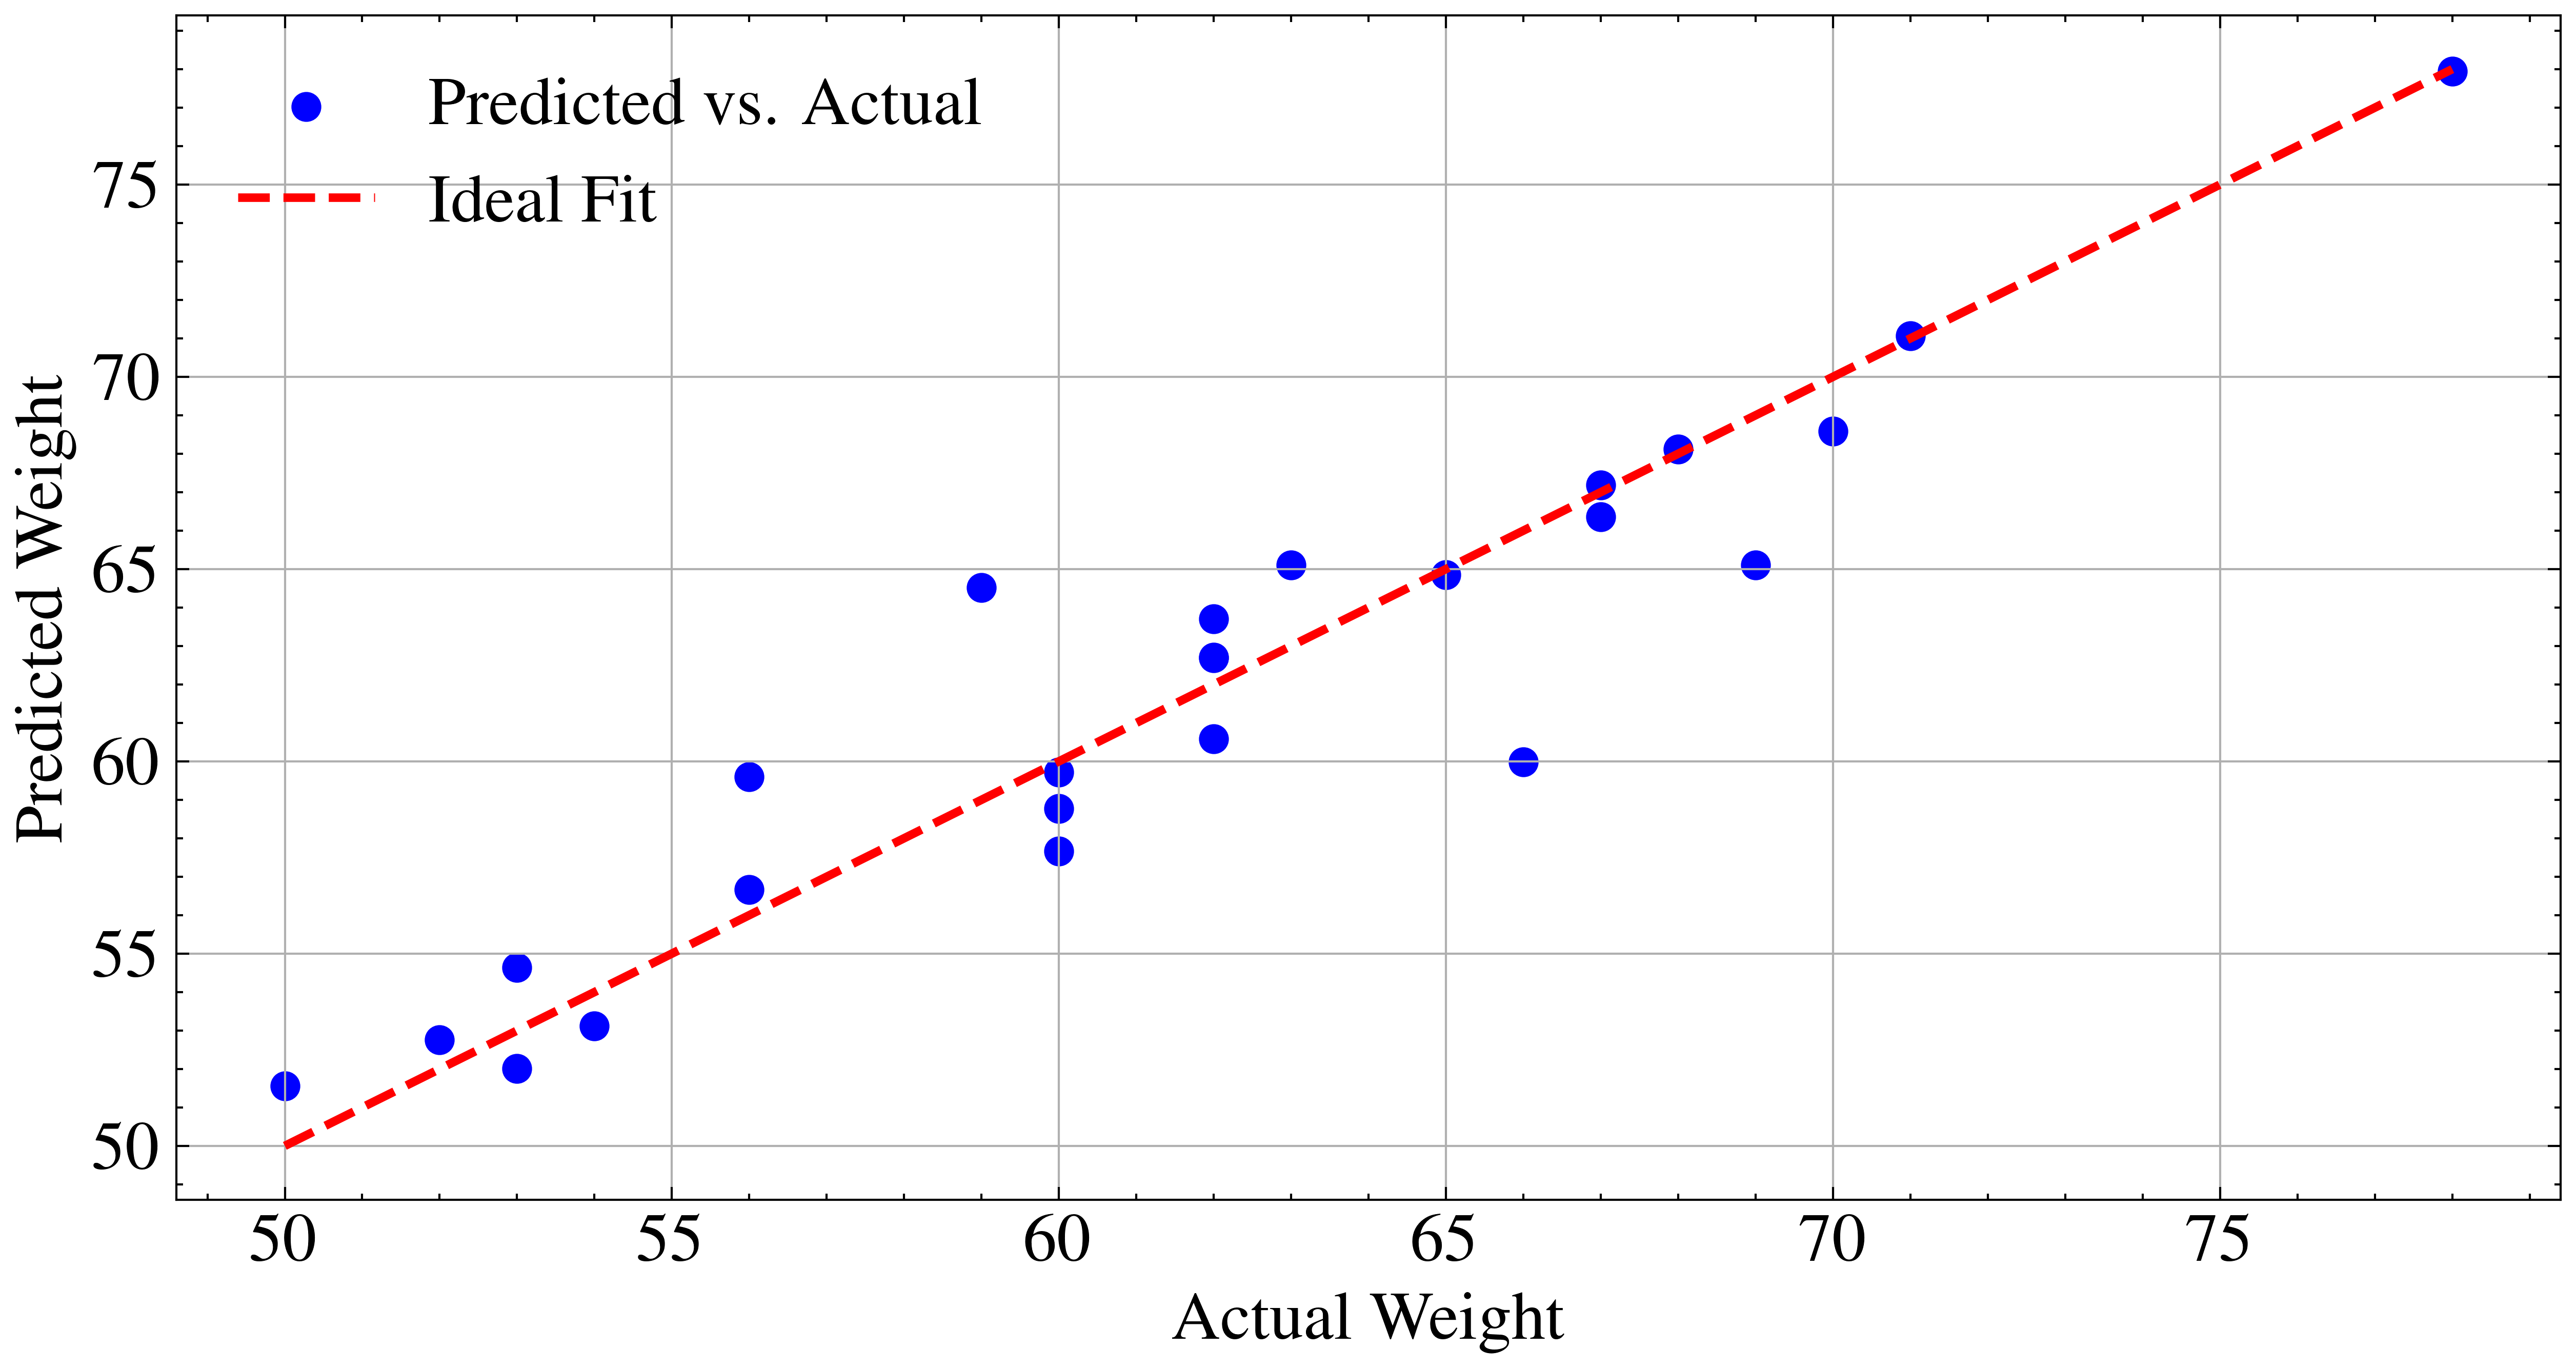
\includegraphics[width=\linewidth]{src/figures/polynominal-regression/polynomial_regression-n-4.png}
        \subcaption{$n=4$}
    \end{subfigure}
    \caption{Polynomial regression with different degrees.}\label{fig:polynomial-regression}
\end{figure}

実際に$n$が増加するにつれて理想的な直線に近づいていることがわかる。
$n$を1から24まで変化させたとき、決定係数の値を表\ref{tab:polynomial-regression}に示す。
$n$を増加させていけば、決定係数が1に近づいていく。
一方で、$n$を増加させすぎると与えられたデータに対して過剰に適合してしまうことがある。
この場合、未知のデータに対しては学習データに比べて損失が大きくなる。
これを過学習などという。
防ぐためには、学習に用いるデータとテストに用いるデータを分け、学習のデータでまずは損失が少なくなるように係数を決定し、
学習とは別にテストデータでモデルにとって未知のデータに対する損失を計算することで過学習を防ぐ適切な次数を選択することができる。
今回はデータ数が少ないため、そこまでは行わない。
\begin{table}
	\caption{多項式回帰の結果} \label{tab:polynomial-regression}
	\centering
	\begin{tabular}{ccc}
		\toprule
		$n$ & $r^2$              & $r$                \\
		\midrule
		1   & 0.7289728080005667 & 0.8537990442724603 \\
		2   & 0.7796704565611795 & 0.8829894996890844 \\
		3   & 0.8009745797898338 & 0.8949718318415579 \\
		4   & 0.8909853059474017 & 0.9439201798602473 \\
		5   & 0.9190776088160172 & 0.9586853544390971 \\
		6   & 0.9198383348695942 & 0.9590820271851591 \\
		7   & 0.9836978240369479 & 0.9918154183299168 \\
		8   & 0.9839301427951513 & 0.9919325293562821 \\
		9   & 0.9839161720140193 & 0.9919254871279491 \\
		10  & 0.9839812723357316 & 0.9919583017121897 \\
		11  & 0.9839751654248222 & 0.991955223497927  \\
		12  & 0.9839778583821335 & 0.9919565808956224 \\
		13  & 0.9839826916460465 & 0.9919590171201865 \\
		14  & 0.9839788579431717 & 0.991957084728554  \\
		15  & 0.9839764686665925 & 0.9919558804032529 \\
		16  & 0.9839717616702413 & 0.9919535078168943 \\
		17  & 0.9839726159581086 & 0.991953938425625  \\
		18  & 0.9839748929279314 & 0.9919550861444945 \\
		19  & 0.9839790371389151 & 0.9919571750528926 \\
		20  & 0.9839832013828491 & 0.9919592740545597 \\
		21  & 0.9839833860295523 & 0.9919593671262711 \\
		22  & 0.9839791219853846 & 0.9919572178200956 \\
		23  & 0.9839827520567327 & 0.9919590475703787 \\
		24  & 0.9839831662691004 & 0.9919592563553709 \\
		\bottomrule
	\end{tabular}
\end{table}


\subsubsection{NBA2022-2023シーズンにおける重回帰分析}
NBA(National Basketball Association)の2022-2023シーズンにおける選手のスタッツのデータを用いて重回帰分析を行う。
データは、Vivo Vinco氏のKaggleのデータセットを用いる。\footnote{
	\url{https://www.kaggle.com/datasets/vivovinco/20222023-nba-player-stats-regular}.
	CC-BY 4.0 ライセンス
}
以下の情報を含む。 Rk,
Player, Pos, Age, Tm, G, GS, MP, FG, FGA, FG\%, 3P, 3PA, 3P\%, 2P, 2PA, 2P\%, eFG\%, FT, FTA, FT\%, ORB, DRB, TRB, AST, STL, BLK, TOV, PF, PTS, TRB, AST, STL, BLK, TOV, PF, PTS
\footnote{
	Rk : Rank,
	Player : Player's name,
	Pos : Position,
	Age : Player's age,
	Tm : Team,
	G : Games played,
	GS : Games started,
	MP : Minutes played per game,
	FG : Field goals per game,
	FGA : Field goal attempts per game,
	FG\% : Field goal percentage,
	3P : 3-point field goals per game,
	3PA : 3-point field goal attempts per game,
	3P\% : 3-point field goal percentage,
	2P : 2-point field goals per game,
	2PA : 2-point field goal attempts per game,
	2P\% : 2-point field goal percentage, ,
	eFG\% : Effective field goal percentage,
	FT : Free throws per game,
	FTA : Free throw attempts per game,
	FT\% : Free throw percentage,
	ORB : Offensive rebounds per game,
	DRB : Defensive rebounds per game,
	TRB : Total rebounds per game,
	AST : Assists per game,
	STL : Steals per game,
	BLK : Blocks per game,
	TOV : Turnovers per game,
	PF : Personal fouls per game,
	PTS : Points per gameTRB : Total rebounds per game,
	AST : Assists per game,
	STL : Steals per game,
	BLK : Blocks per game,
	TOV : Turnovers per game,
	PF : Personal fouls per game,
	PTS : Points per game
}
これらのデータの中から、まず
Age, Pos, MP, FG, FGA, FG\%, 3P, 3PA, 3P\%, FT, FTA, FT\%を説明変数とし、
PTSを目的変数として重回帰分析を行う。
今回は学習データとテストデータをわけ、学習データでモデルを構築し、テストデータでモデルの性能を評価する。
決定係数は$0.9998950394227705$となり非常に高い精度で予測ができていることがわかる。
予測した値と実際の値の比較を図\ref{fig:actual-vs-predicted-PTS}に示す。
シュートに関するほぼ全ての統計量を説明変数とし、
得点を目的変数としているからのかなり高い精度で予測できたと考えられる。
\begin{figure}
	\centering
	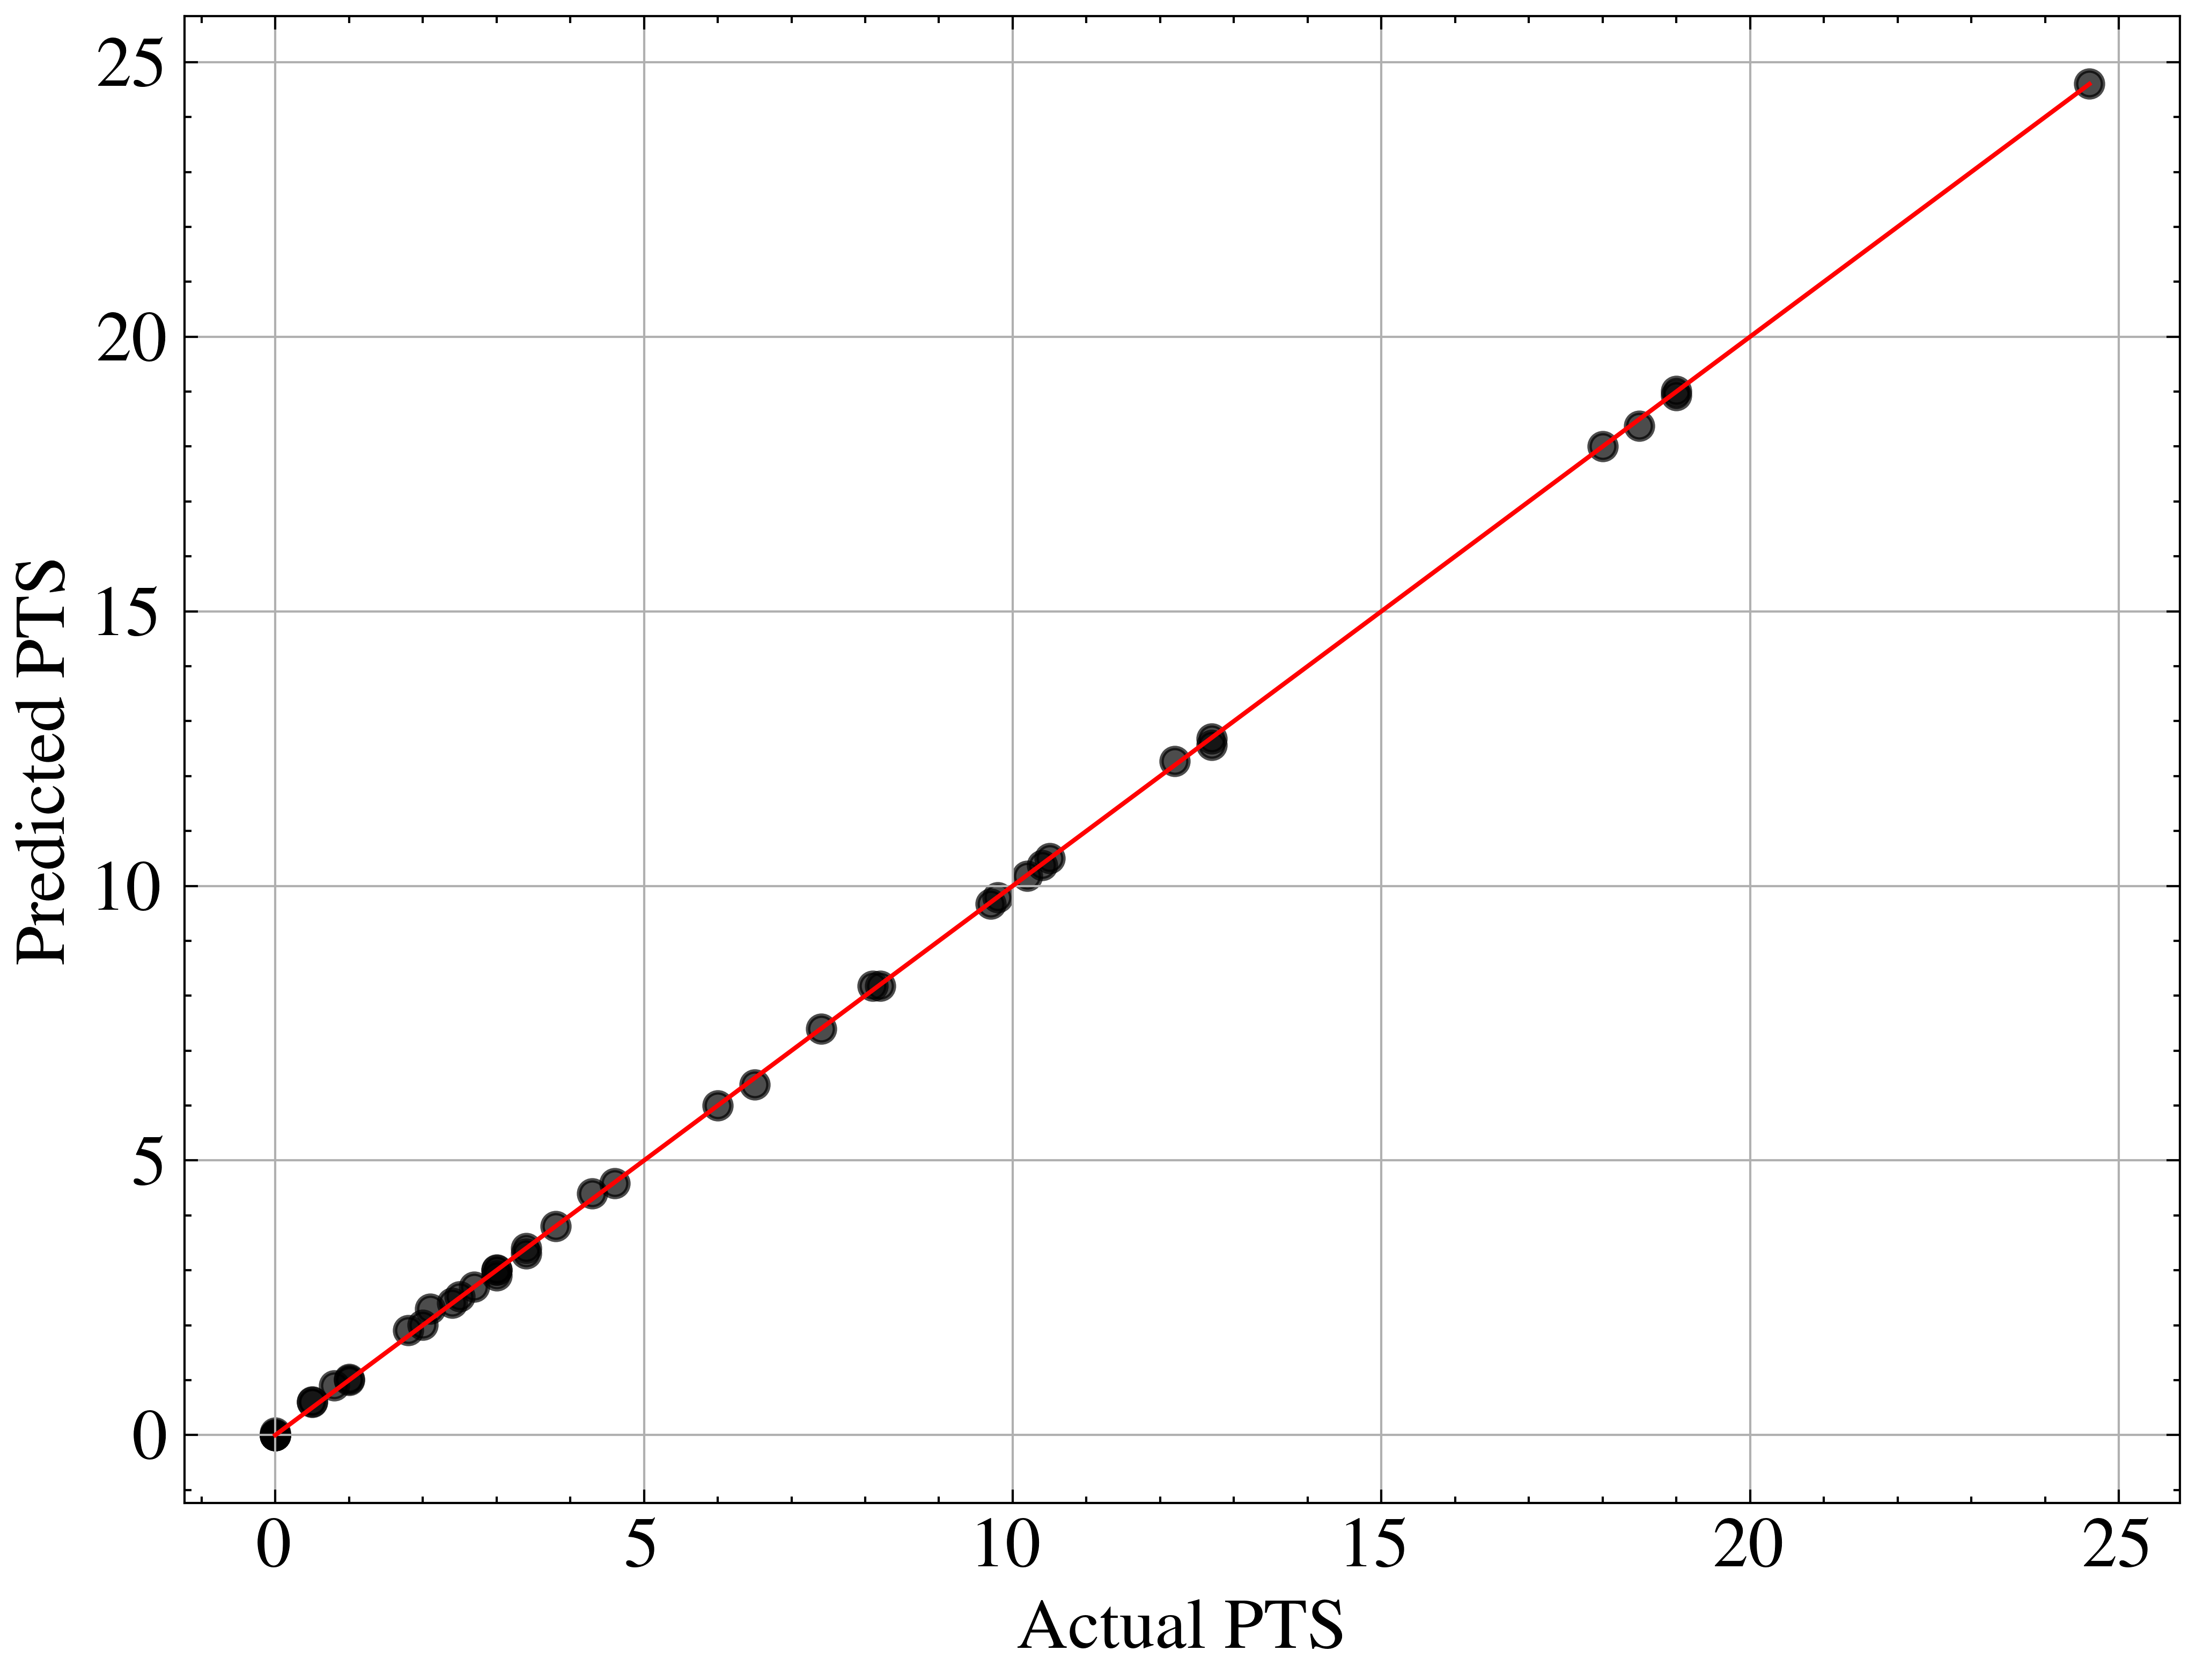
\includegraphics[width=0.8\linewidth]{src/figures/nba-regression/actual-vs-predicted-PTS.png}
	\caption{実際の得点と予測された得点の比較}\label{fig:actual-vs-predicted-PTS}
\end{figure}


一方で、MP, Age, STL, BLKを説明変数としPTSを目的変数とすると、
決定係数は$0.787534156007302$となり上記の場合に比べて低くなっている。
これは、FGに関する情報、FTに関する情報などを説明変数とせず、PTSに直接関係のないような
AgeやMP、STL、BLKを説明変数としているためであると考えられる。
\begin{figure}
    \centering
    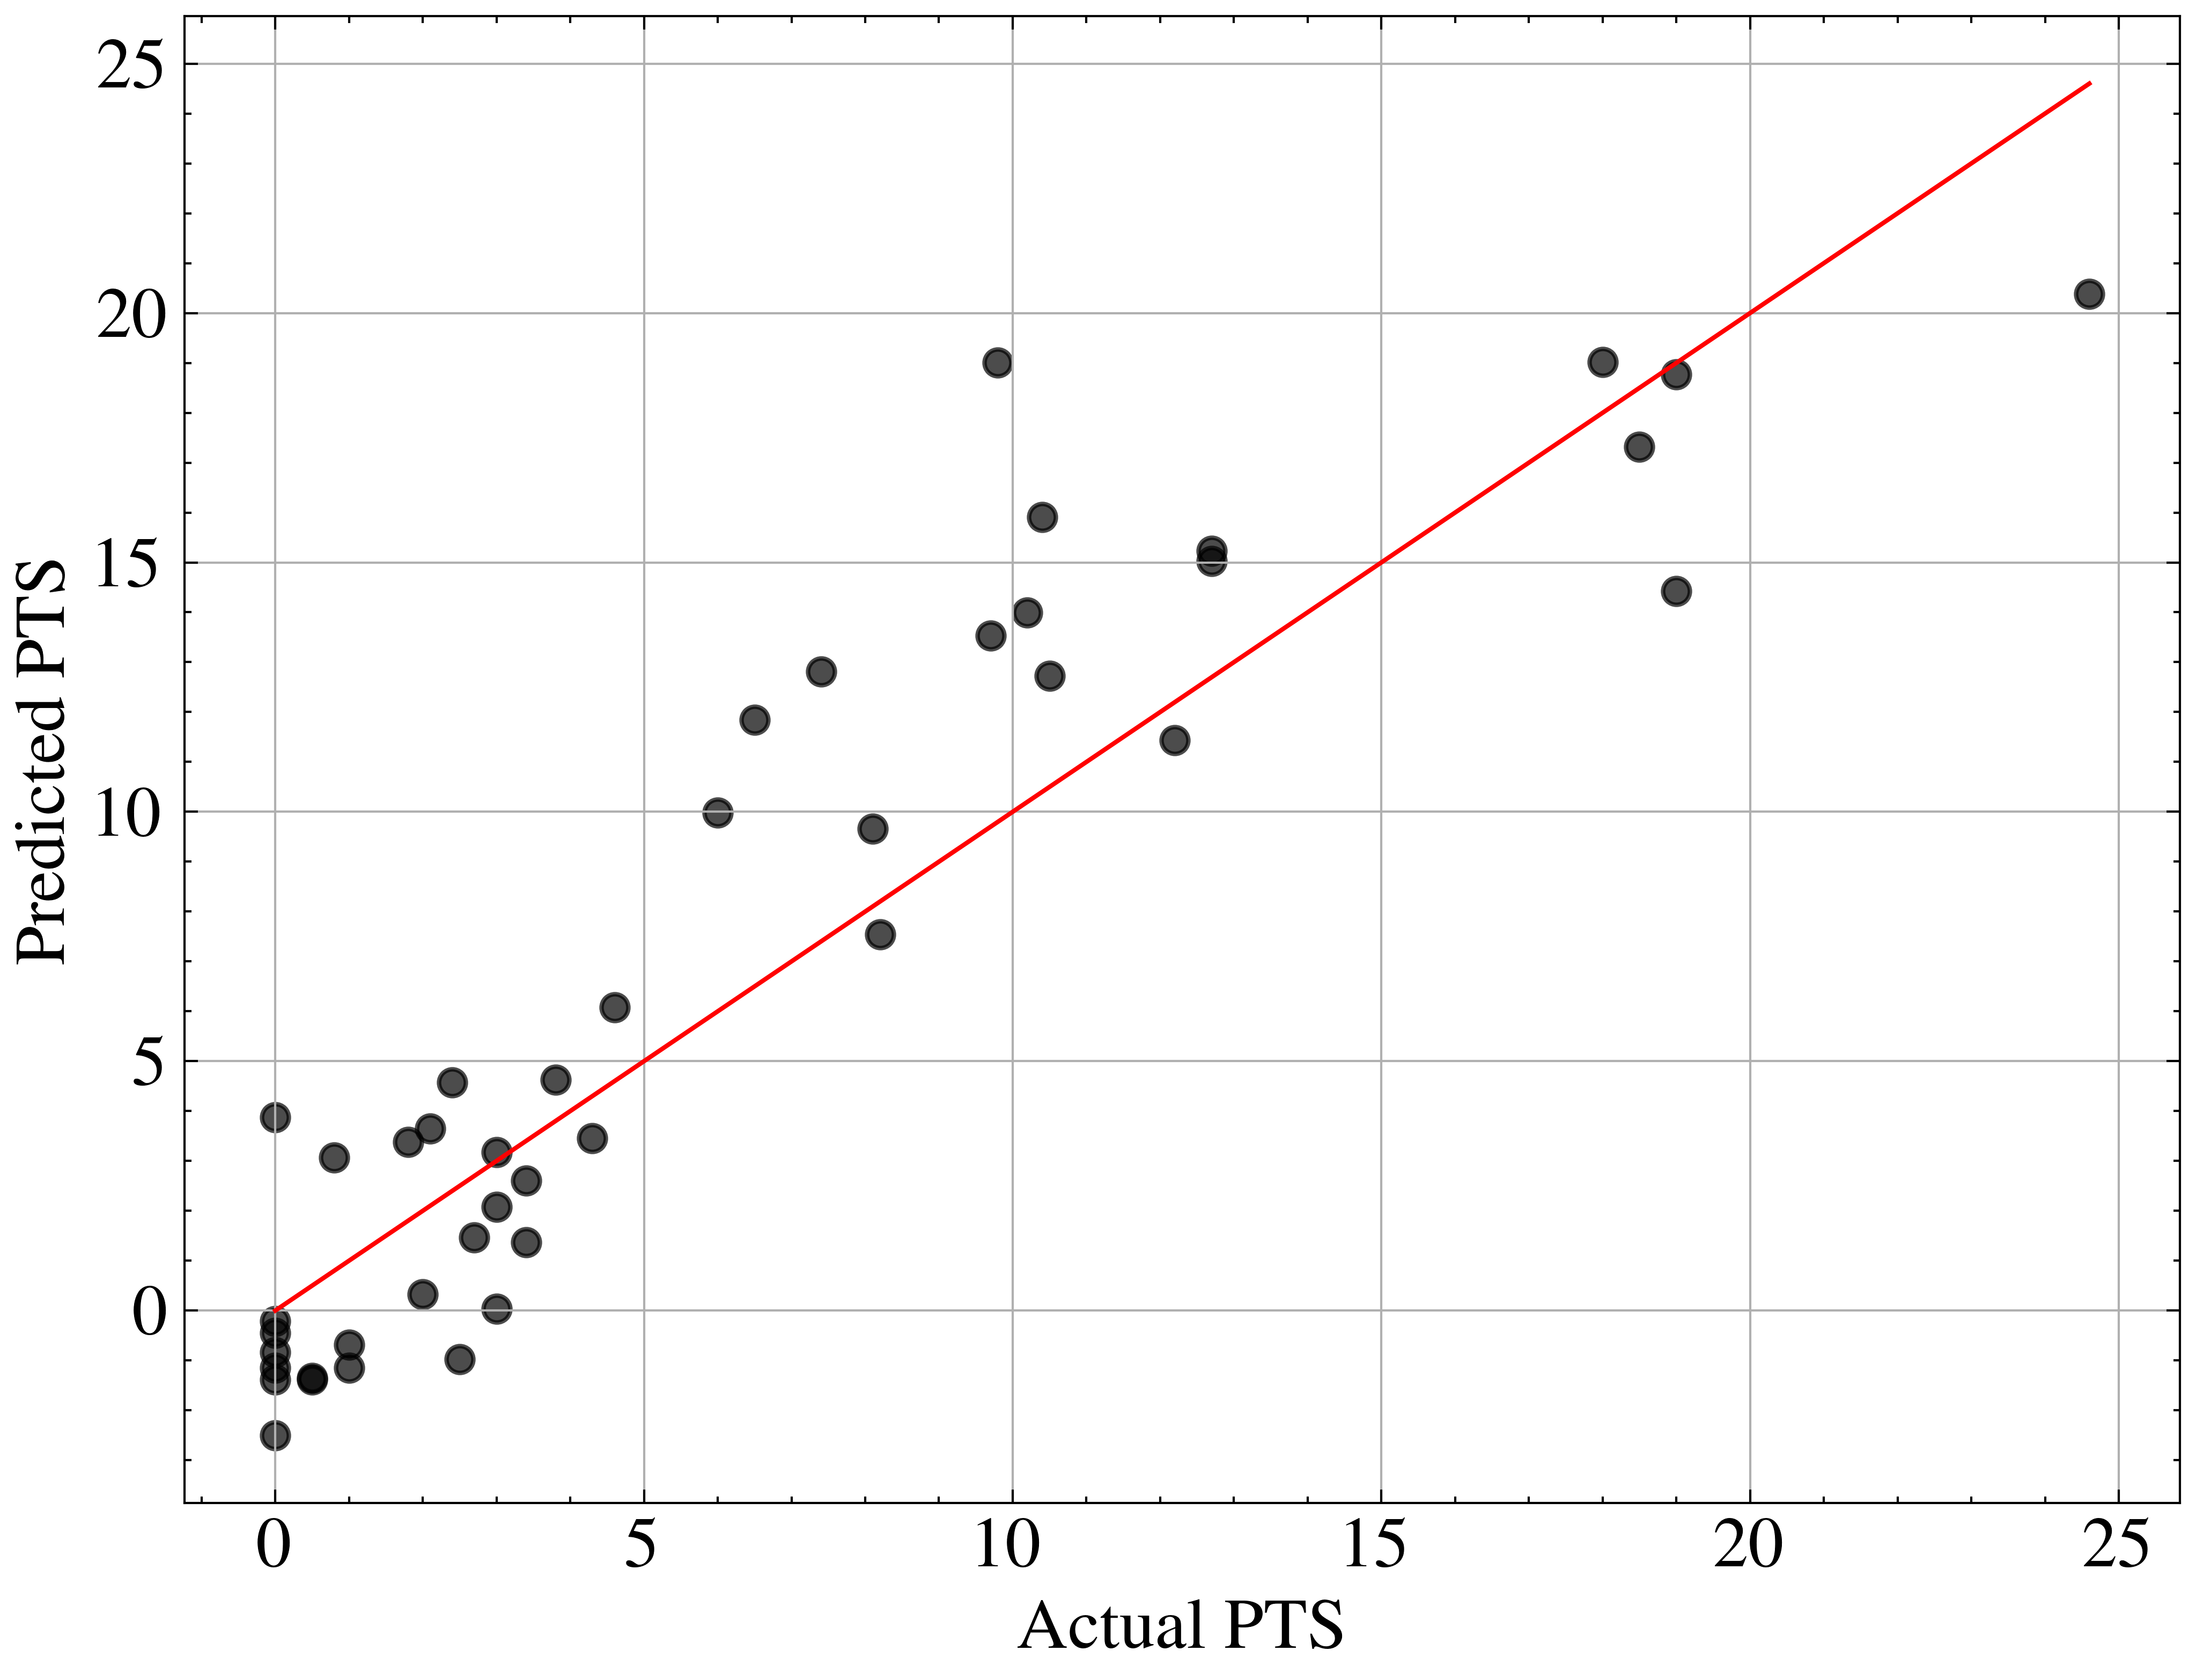
\includegraphics[width=0.8\linewidth]{src/figures/nba-regression/actual-vs-predicted-PTS-2.png}
    \caption{実際の得点と予測された得点の比較}\label{fig:actual-vs-predicted-PTS-2}
\end{figure}


PTS以外の全ての統計量を説明変数としPTSを目的変数とすると、決定係数は$0.999872848991546$となりはじめの場合に比べてやや高くなっている。
一方で、得点を説明するのはAge, Pos, MP, FG, FGA, FG\%, 3P, 3PA, 3P\%, FT, FTA, FT\%などで十分と考えられ、
それ以外の統計量はただ不要なパラメータを増やし計算量を増やすだけである。
したがって、上記のように目的変数に対してどういう説明変数が関連しているか適切に判断し選択することが大事である。


\end{document}
